\documentclass[twoside,a4paper,twocolumn,10pt]{article}

\usepackage[margin=2cm]{geometry}
\usepackage{amsmath,amsthm,amssymb,latexsym}
\usepackage{graphicx}
%\usepackage{backref}

\theoremstyle{plain}
\newtheorem{proposition}{Proposition}[section]
\newtheorem{theorem}[proposition]{Theorem}
\newtheorem{corollary}[proposition]{Corollary}
\newtheorem{lemma}[proposition]{Lemma}
\theoremstyle{definition}
\newtheorem{definition}[proposition]{Definition}
\newtheorem{remark}[proposition]{Remark}
\newtheorem{example}[proposition]{Example}
\newtheorem{conjecture}[proposition]{Conjecture}

%\newcommand{\rd}{\textrm{d}}
\newcommand{\regsym}{\textsuperscript{\textregistered}}

\begin{document}

\title{Open crime data-sets: Pitfalls of geocoding}
\author{Matthew Daws}
\maketitle

\begin{abstract}
The rise of Open Data has lead to the release, especially in the USA, of rich
crime datasets, often with seemingly precisely coded geographical locations.
These datasets are increasingly being used by researchers; we are particularly
interested in the design and evaluation of predictive policing algorithms.
We present a case study of data from a number of US cities, exploring some of
the problems with naively assuming that the data is correct ``as is''.  We develop
novel algorithms for reassigning location points in a more ``realistic'' manner,
operating both in two dimensional space, and on the street network.
The software used is released in an Open Source manner,
in the hope that other researchers can directly use, and also extend, the work,
with minimal extra effort.
\end{abstract}


\section{Introduction}

This study arose from our interest in spatial ``predictive policing'' algorithms,
see \cite{rand} for an overview of this field.  We have implemented a number of
common predictive algorithms in an open source Python package,
\texttt{open\_cp}, \cite{opencp}.
However, algorithms are only one part of the equation: data is also needed to make
predictions from, and to assess predictions against.

Working in the UK, and partnered with a police force, we have private access to,
for example, Burglary crime events in West Yorkshire.  In our case, such data has a
number of interesting features:
\begin{itemize}
\item Each crime event is precisely geo-coded to longitude and latitude coordinates
  which appear to correspond to the centroid of building locations.  The UK is fortunate
  in having the UK Ordnance Survey, a publicly owned company, which provides a de facto
  standard for mapping and geolocation.  From speaking to people involved in the creation
  of the data, much of the geocoding occurs by hand after the crime is reported.
\item Each crime event comes with a ``report'' timestamp, and also an estimate of the
  time range in which the crime could have occurred.  (For example, with burglary, the
  crime is often discovered when the property owner returns to the property, and so an
  exact time when the event occurred cannot be known; see \cite{ratcliffe}.
  From our analysis, such data is somewhat noisy, with the time range often being meaninglessly
  short, or even impossible.
\end{itemize}
Such a dataset is a valuable resource to researchers, but it also has problems.  The data
is private, and cannot be shared with other researchers.  This makes reproducing any
research extremely hard.  Furthermore, the data relies upon other
commercial products: for example, the geocoding seems to exactly correspond to data
from the Ordnance Survey ``MasterMap'' product, which is commerical, and not available
free of charge to the public.  Notice also our description of certain errors, or sources of
possible bias, in the geocoding and timestamps.

Police forces in the UK release summary data, available from \texttt{https://data.police.uk/}.
This data is an incredibly large and useful source of \emph{aggregated} data, but the timestamps
are \emph{months} only, and the locations are partly anonymised, to quote:
\begin{quote}
Each map point is specifically chosen so that it:
\begin{itemize}
\item Appears over the centre point of a street, above a public place such as a Park or Airport, or
  above a commercial premise like a Shopping Centre or Nightclub.
\item Has a catchment area which contains at least eight postal addresses or no postal addresses at all.
\end{itemize}
\end{quote}
The timestamp issue, in particular, means that this data is not suitable for use with
short-range crime prediction algorithms.

In the USA, similar data is available from \texttt{https://www.data.gov/}, often with very
rich (which is to say, seemingly ``accurate'') timestamps and geographical location data,
and helpful additional metadata about the crime events.  However,
the decentralised nature of government in the USA leads a number of problems:
\begin{itemize}
\item There appears to be no central standard, or even a common set of guidelines,
  as to how to produce data.  The three datasets we study here are very different.
\item There is rather little information as to how the datasets are produced.  The quote
  above from the UK police dataset clearly explains how the given geographical coordinates
  relate to ``reality''.  We have not found such guidance for the datasets we study here.
\end{itemize}

We used above the term ``Open Data'', which is a loosely defined term, see \cite{odi}
for example.  Our usage will be colloquial, and less strict than \cite{odi}; in particular,
we mean data that is free to download, but our data may have certain usage restrictions
placed upon it.

It is important to remember that just because data is ``open'', it does not mean that it
corresponds exactly to reality.  As \cite{econ1} reminds us, crime statistics in particular
can be subject to political pressure at a much higher level than ``geocoding''!
For examples of academic papers using the Chicago data, see \cite{eftelioglu}, \cite{rosser_sepp},
\cite{hlo}.  Internet searches will find many online ``data science'' resources using this
dataset.  We are not aware of any systematic exploration of the geo-coding.  The San Francisco
and Dallas datasets appear to have been used less in academic work; we chose them as they offer
a contrast to the Chicago data in various ways.

We have found rather little in the literature about the effects of the input data on
the output of crime prediction algorithms.  However, an excellent survey article is \cite{HZ}.
This paper
concentrates upon geocoding, by police, of crime events, and provides some recommendations.
It gives a summary of other research suggesting that KDE methods are likely to be impacted by
poor quality geocoding.  This paper also considers prediction techniques, and concludes:
\begin{quote}
The effect of geocoding quality on predictive hotspot mapping is complex and varies depending on prediction
technique (and parameter settings within them), crime type, and urban morphology.
\end{quote}
We are not aware of any similar study for openly available data, and so we hope this
paper fills a much needed gap.



\subsection{Organisation of the paper}

We have three main aims in this study.  Firstly, we wish to \emph{document} how we worked
with the data, and show some of the patterns we have found.  None of the above papers
which use the (for example, Chicago) data seem
to have discussion of the data at all, and use the data in a perhaps uncritical way.
(There might, for example, be systematic biases which could affect results.  Or there might not.
But without looking carefully, it is hard to know).  We will find that in all cases, the
geographical coordinates are not accurate, and often have systematic randomisation or aggregation
applied.  We develop some algorithms to randomly move coordinates so as to produce more
``realistic'' geocodings, or at least less systematically biased locations.  Finally, we
have implemented all the code in an open source Python package.  This will allow other researchers
to very quickly load and manipulate data from the three sources we study; the algorithms can be
applied to any dataset which can be manipulated into the correct form; it should be relatively
easy to adapt the code to other, similar datasets.

We strongly believe in the need for \emph{reproducible research}, \cite{hl, morin}.
Beyond publishing computer code, \cite{barnes}, it is also important to detail how data was collected
and processed: this is an important aim of this paper.  Within the framework of
Geographic Information Science, we believe in the aims of \cite{ssb}: in particular, the
importance of using a high-level, though general purpose, programming language, to fully
document all the steps taken in the spatial analysis; contrast this with using a graphical
GIS where it is extremely hard to document exactly which steps were taken by the researcher.

Our computing environment is Python~3.5+.  We have developed a package \texttt{opencrimedata}
which can be installed from the GitHub repository \cite{ocd}.
This provides a simple API to load the data from the datasets into Python, and a high-level
API to perform various ``redistribution tasks'', see Section~\ref{sec:reassign}.
All figures in this paper were produced using Jupyter Notebooks which may also be downloaded from
the GitHub repository.  Finally, the repository contains a number of further notebooks which may
be of interest.

We have found it useful to \emph{both} develop a Python package, and use notebooks.
By working with straight Python, we can adopt a test-driven development approach, \cite{beck},
and carefully develop moderately complicated algorithms while testing them.  We also provide
\texttt{pydoc} documentation on the classes and functions developed: these can be displayed
interactively in a notebook, and we have found this to be an excellent way of remembering
how our code works, without the need to re-read the actual source code.  Notebooks then provide
a great way to visualise the output of algorithms, and to provide additional documentation.
Compared to just writing Python code in a notebook, our approach leads to better tested code,
far less repetition, a cleaner API, and uncluttered notebooks.  It also allows much easier
re-use of the underlying algorithms: you can, for example, load and filter input data in a
single line of Python code (once the package is imported), instead of having to adapt 10s
or 100s of lines of code in a notebook.



\subsection{Acknowledgements}

This work was partly funded by the UK Home Office Police Innovation Fund, through the
project ``More with Less: Authentic Implementation of Evidence-Based Predictive
Patrol Plans''.



\section{Chicago data}

This data is available at \cite{cdata}, and is fairly continuously updated.  Our analysis has been
performed using data covering the period from 1st January 2001 to 9th August 2017 inclusive.
We also make use of the community area boundaries available from \cite{cgeo}.  Later, when we discuss
road networks, we have used the 2016 TIGER/Lines\regsym data from \cite{tiger}, as well
as the Chicago specific data from \cite{cstreets}.

The data comes as a CSV file (and is also available as a yearly snapshot, containing the
same data, in a slightly different format).  Each row has a unique \texttt{ID} number, and
a \texttt{Case Number} which is very nearly unique.  There is no obvious pattern in the repeats
of case numbers, excepting that all ``Homicide'' crimes seem to appear multiple times.
Each row contains information about the ward, community area, police district etc. which
the crime occurred in.  Of interest to us is the following data:
\begin{enumerate}
\item Fields \texttt{Primary Type} and \texttt{Description} which contain the main crime type,
such as ``Burglary'', and a further description, such as ``Forcible entry''.  There are a relatively
small number of unique strings which can occur.
\item Field \texttt{Location Description} which is a string describing the location of the
event, for example ``Abandoned building'' or ``Sidewalk''.  There are 174 choices (including
an empty string).
\item Field \texttt{Block} which is a street name and partly obscured address, such as
``087XX S KINGSTON AVE''.
\item Field \texttt{Date} which contains a date and time, to seconds resolution.
\item A number of fields containing coordinates.  The longitude and latitude are given twice,
and $x,y$ coordinates are given.  These are the projected coordinates, using EPSG:2790, in
units of US Survey feet, and rounded to the nearest foot.  The data is consistent with
either the longitude and latitude being primary and the projected coordinates being calculated
and rounded to the nearest foot, or vice versa.
\end{enumerate}



\subsection{Geo-coding}

The official information about the dataset is very brief, and contains almost no information about
how the data is geocoded beyond:
\begin{quote}
``All data visualizations on maps should be considered approximate and
attempts to derive specific addresses are strictly prohibited.''
\end{quote}
Two plots of the data are shown in Figure~\ref{fig:one}.  Here and elsewhere, the basemap is
``\textcopyright OpenStreetMap contributors'', see \cite{osm}, and rendered using the
\texttt{TileMapBase} Python package, \cite{tmb}.  The extract plot is typical of any visualisation
of the data-set (throughout this work, we have found that a combination of Jupyter Notebooks running
Python has allowed for \emph{reproducible} results to be found, but that using a GIS system,
such as QGIS, \cite{qgis}, for interactive visualisation, is also very profitable).  In particular,
we note:
\begin{itemize}
\item Almost all event locations seem to ``cluster'' to the middle of a street;
\item There are a few ``outliers'': single events a bit away from others;
\item There are a few events which seem to occur just off the middle of the street.  Further
  investigation finds that all of these are events which occurred in 2001; data from 2002 and
  later is always ``clustered'', and data from 2001 never is.
\end{itemize}

\begin{figure*}
  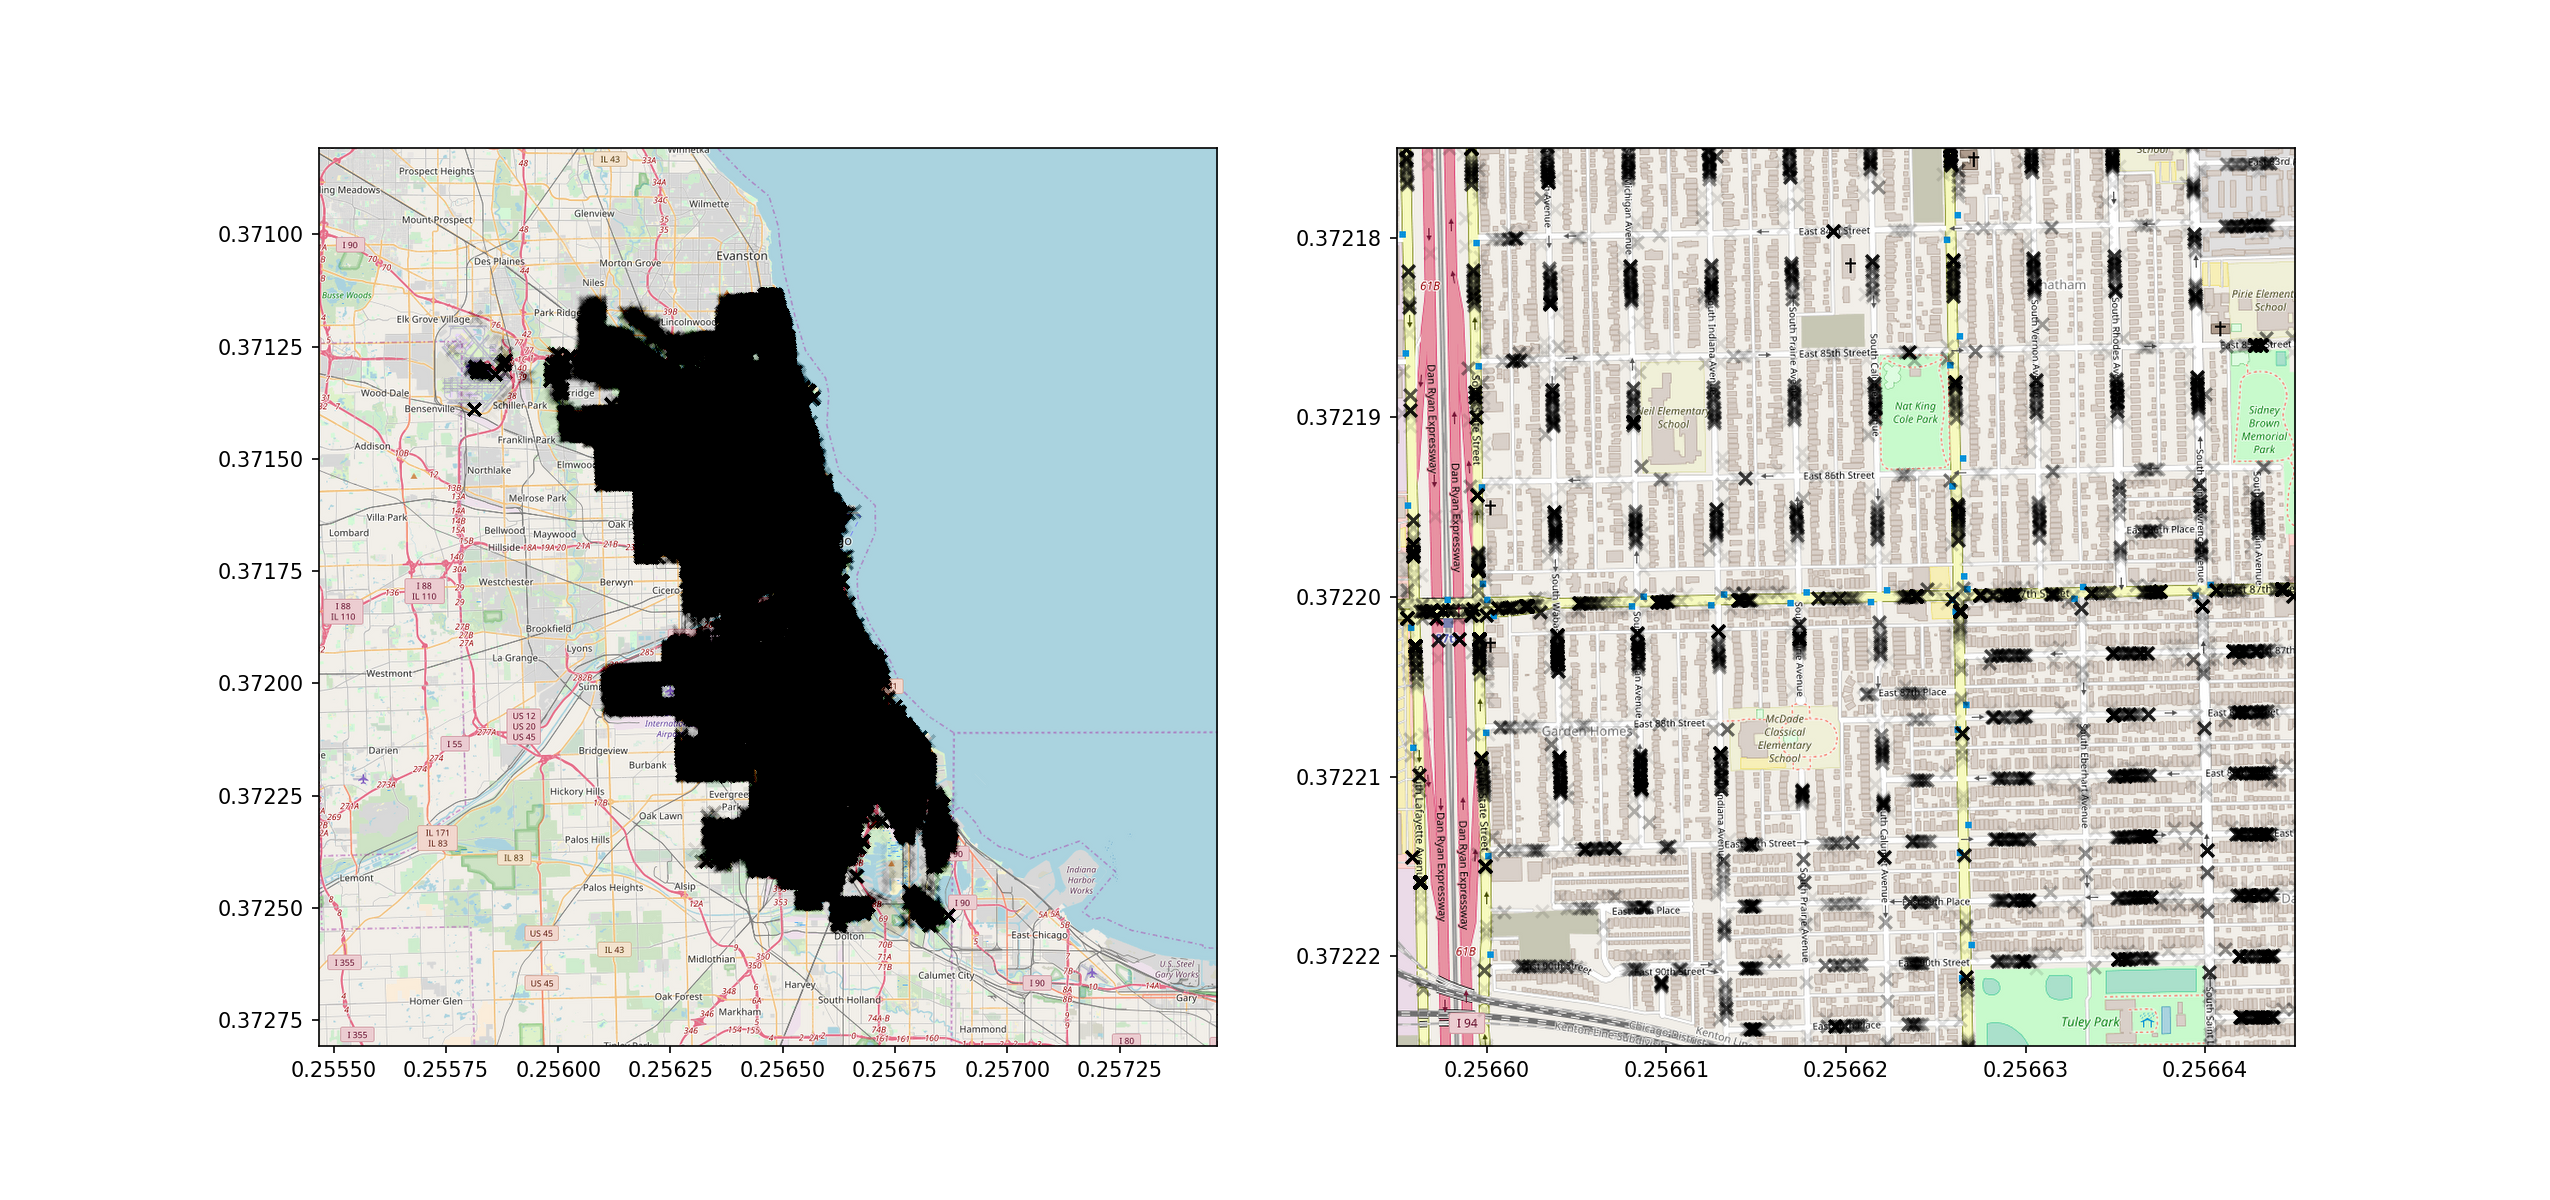
\includegraphics[width=\textwidth]{Chicago_overview.png}
  \caption{The complete Chicago dataset, and an extract showing a typical ``clustering'' of events.}
  \label{fig:one}
\end{figure*}

If one compares these plots with e.g. \cite[Page~3]{rosser_sepp} then they appear to be
different: the plots in \cite{rosser_sepp} seem to show less clustering, and do not exactly
align with the streets on the basemap.  From asking colleagues, we obtained a copy of the
Chicago data downloaded in the middle of 2014, and containing events from 2001 through to
the 24th May 2014.  The geocoding appears to be different in this ``old'' file,
as compared to the ``new'' file.

Given both data-sets, we compared them by linking against the unique id number.  The vast majority
of the records match up, with the exception that the \texttt{Description} field (giving the
``sub-type'' of the crime) changes quite a lot.  We look at only events where the main crime
type does not change, and look at the old and new coordinates.  Firstly, we find that for
events with a timestamp in 2001, except for a very small number of cases
(558 out of 482713 records), the coordinates do not change.

For post-2001 data, excepting a few outliers
(where we conjecture that the address has somehow been corrected) the locations are very close,
but differ in a systematic way.  Figure~\ref{fig:three} illustrates this.  For a single block,
we see that the ``new'' coordinates appear to have been generated from the ``old'' coordinates
by projecting onto the middle of the road, and then ``squashing'' the point together to form
a cluster.  In the second plot, notice how the ``old'' coordinates do not seem to cluster at
all, but form continuous lines along either side of the road.

\begin{figure*}
  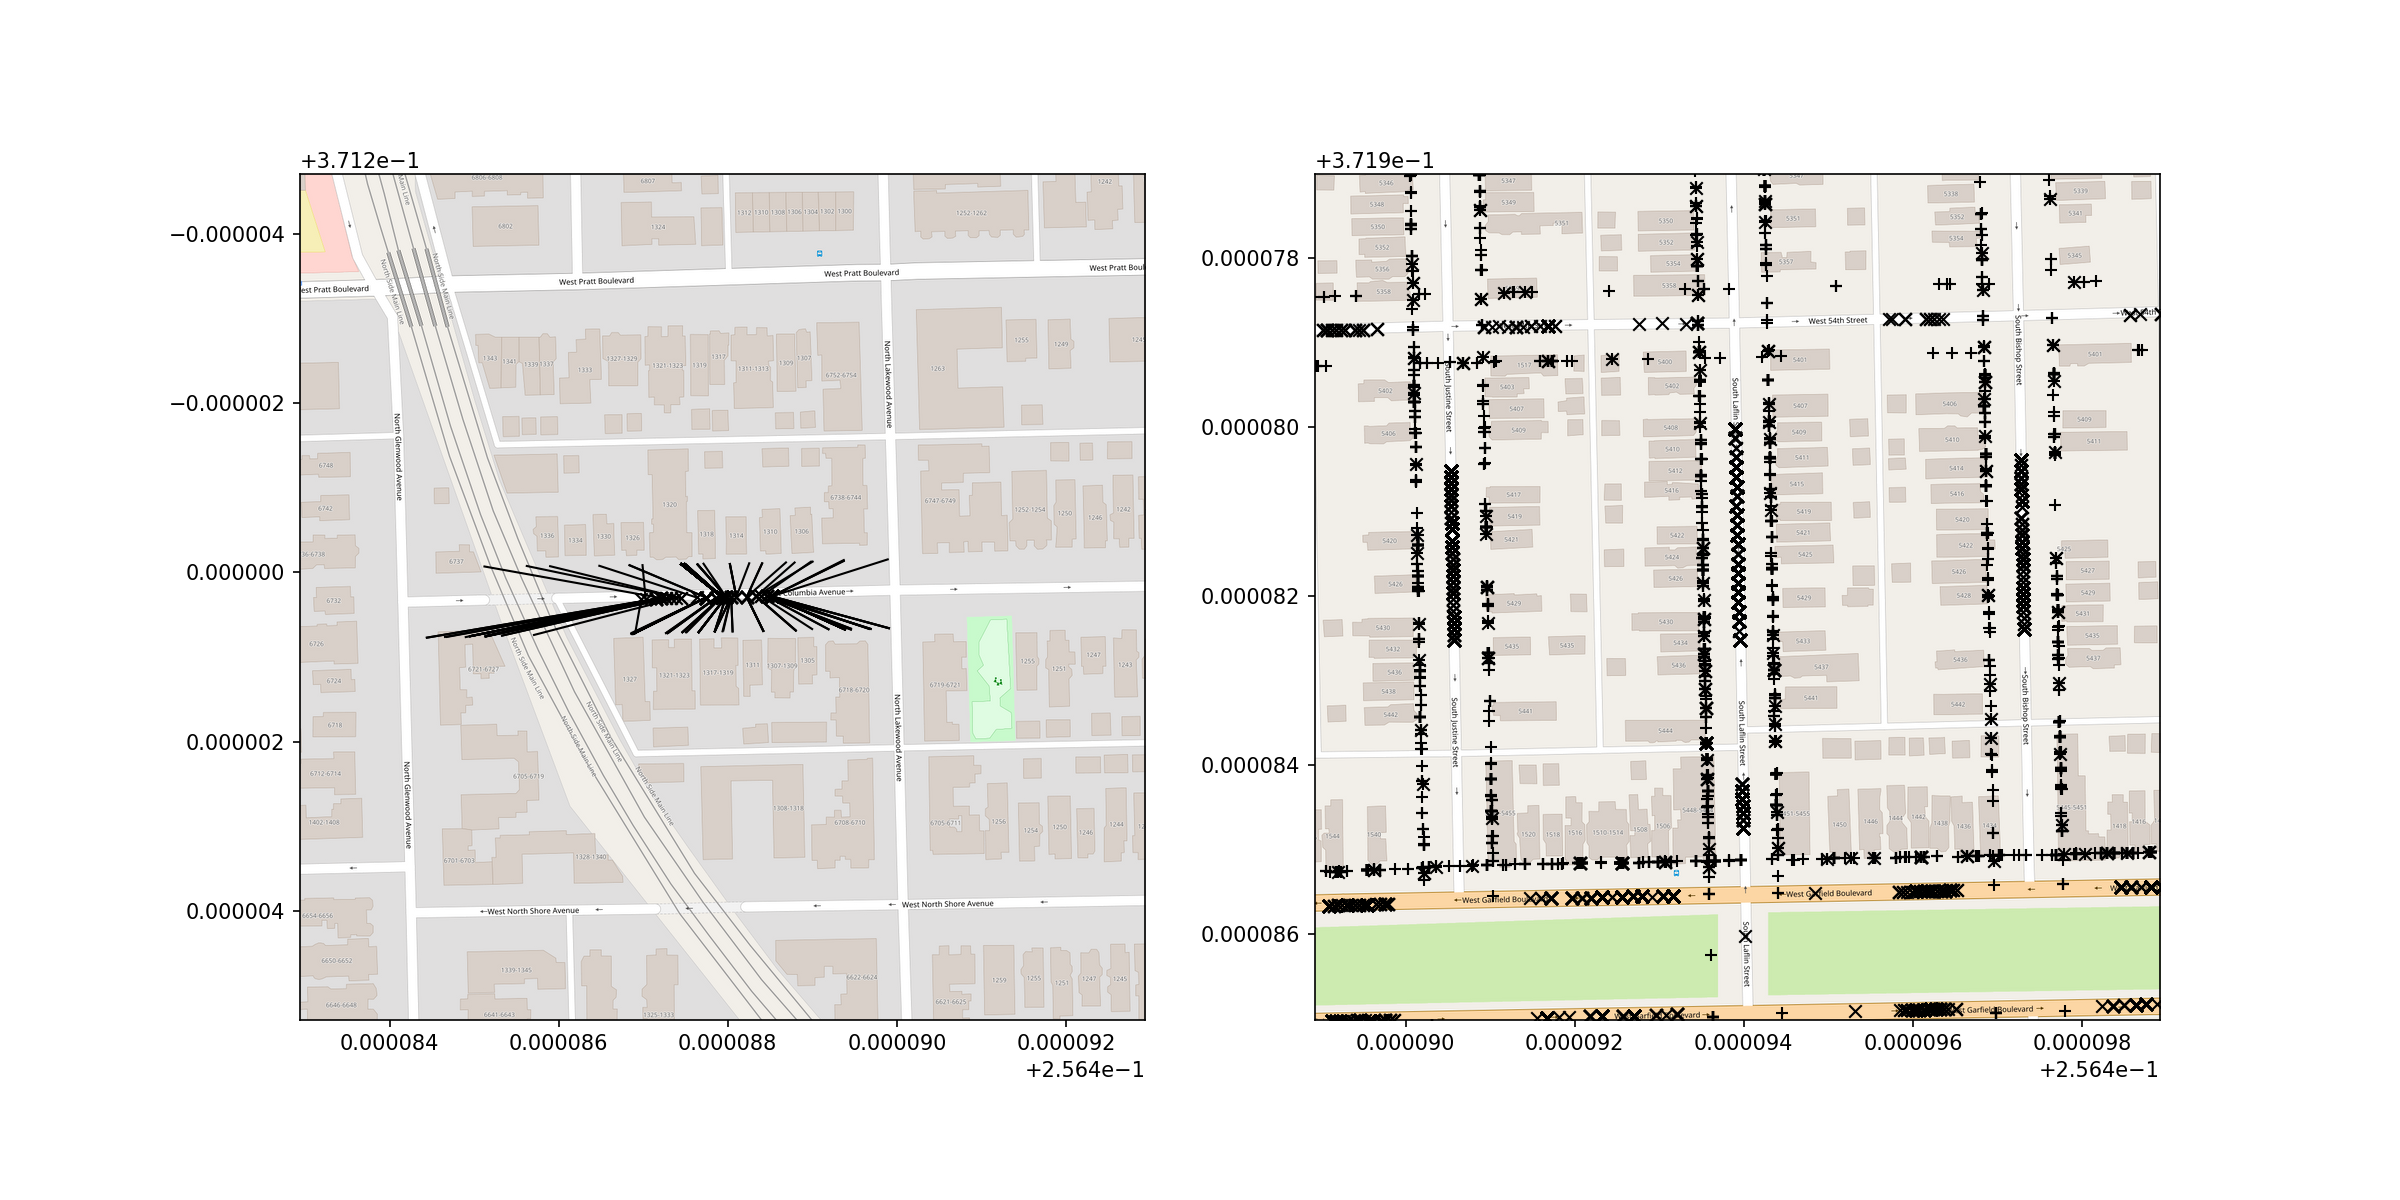
\includegraphics[width=\textwidth]{Chicago_example1.png}
  \caption{To left, a plot of the data with block ``013XX W COLUMBIA AVE'', lines joining the
``old'' and ``new'' coordinates.  To right, same for ``054XX S LAFLIN ST'', but with surrounding
blocks drawn as well.  ``new'' coordinates are also marked with a ``x'', and ``old'' coordinates
with a ``+''; we see the split between 2001 and post-2001 data.}
  \label{fig:three}
\end{figure*}

The base map is from OpenStreetMap, and there is a \emph{superficial} alignment between the
``old'' points and the outlined buildings.  However, a more systematic look will show that the
``old'' points always appear in two lines, directly parallel to the street.  It is extremely
far from the case that there is a one-to-one correspondance between points and buildings:
many points seem unconnected to any building, while a single building might have many points
close to it.  There appear to be no events which occur close to alleyways or footpaths or other
minor roads (although clearly crime \emph{must} happen in these locations) nor near to
buildings not close to streets.

In summary, we do not believe that there is any real correspondence between the ``old'' points
and the actual location of the crime.  It appears much more likely that the points are
automatically and randomly generated from the ``Block'' on which the crime is logged against.

This said, there does appear to be some real information in the side of the street which the
``old'' points occurs on, see Figure~\ref{fig:four}.  Here we show two blocks, one north
of the other.  To observe is the way the blocks overlap: the most southerly points only
occur to the left, while in the overlap, the points associated to the 6500 block occur
to the right, and those associated to the 6600 block occur to the left.
If we check the actual addresses of building in this area, then this agrees with
reality-- for that section of street, the left side is in the 6600 block, and the right
side in the 6500 block.

There is a church prominently in these two plots.  We looked at the ``Location'' field
and those events which claim to have happened on church property.  These do indeed seem
to cluster close to the church, with a couple of other events further away.  What we
do not see is events claiming to be from the church uniformly distributed all along
the ``block''.  We looked at all events with a location of a church, and explored these
using QGIS.  They appear to be clustered in a similar way, with a close, but far from
exact, alignment with actual places of worship.

\begin{figure*}
  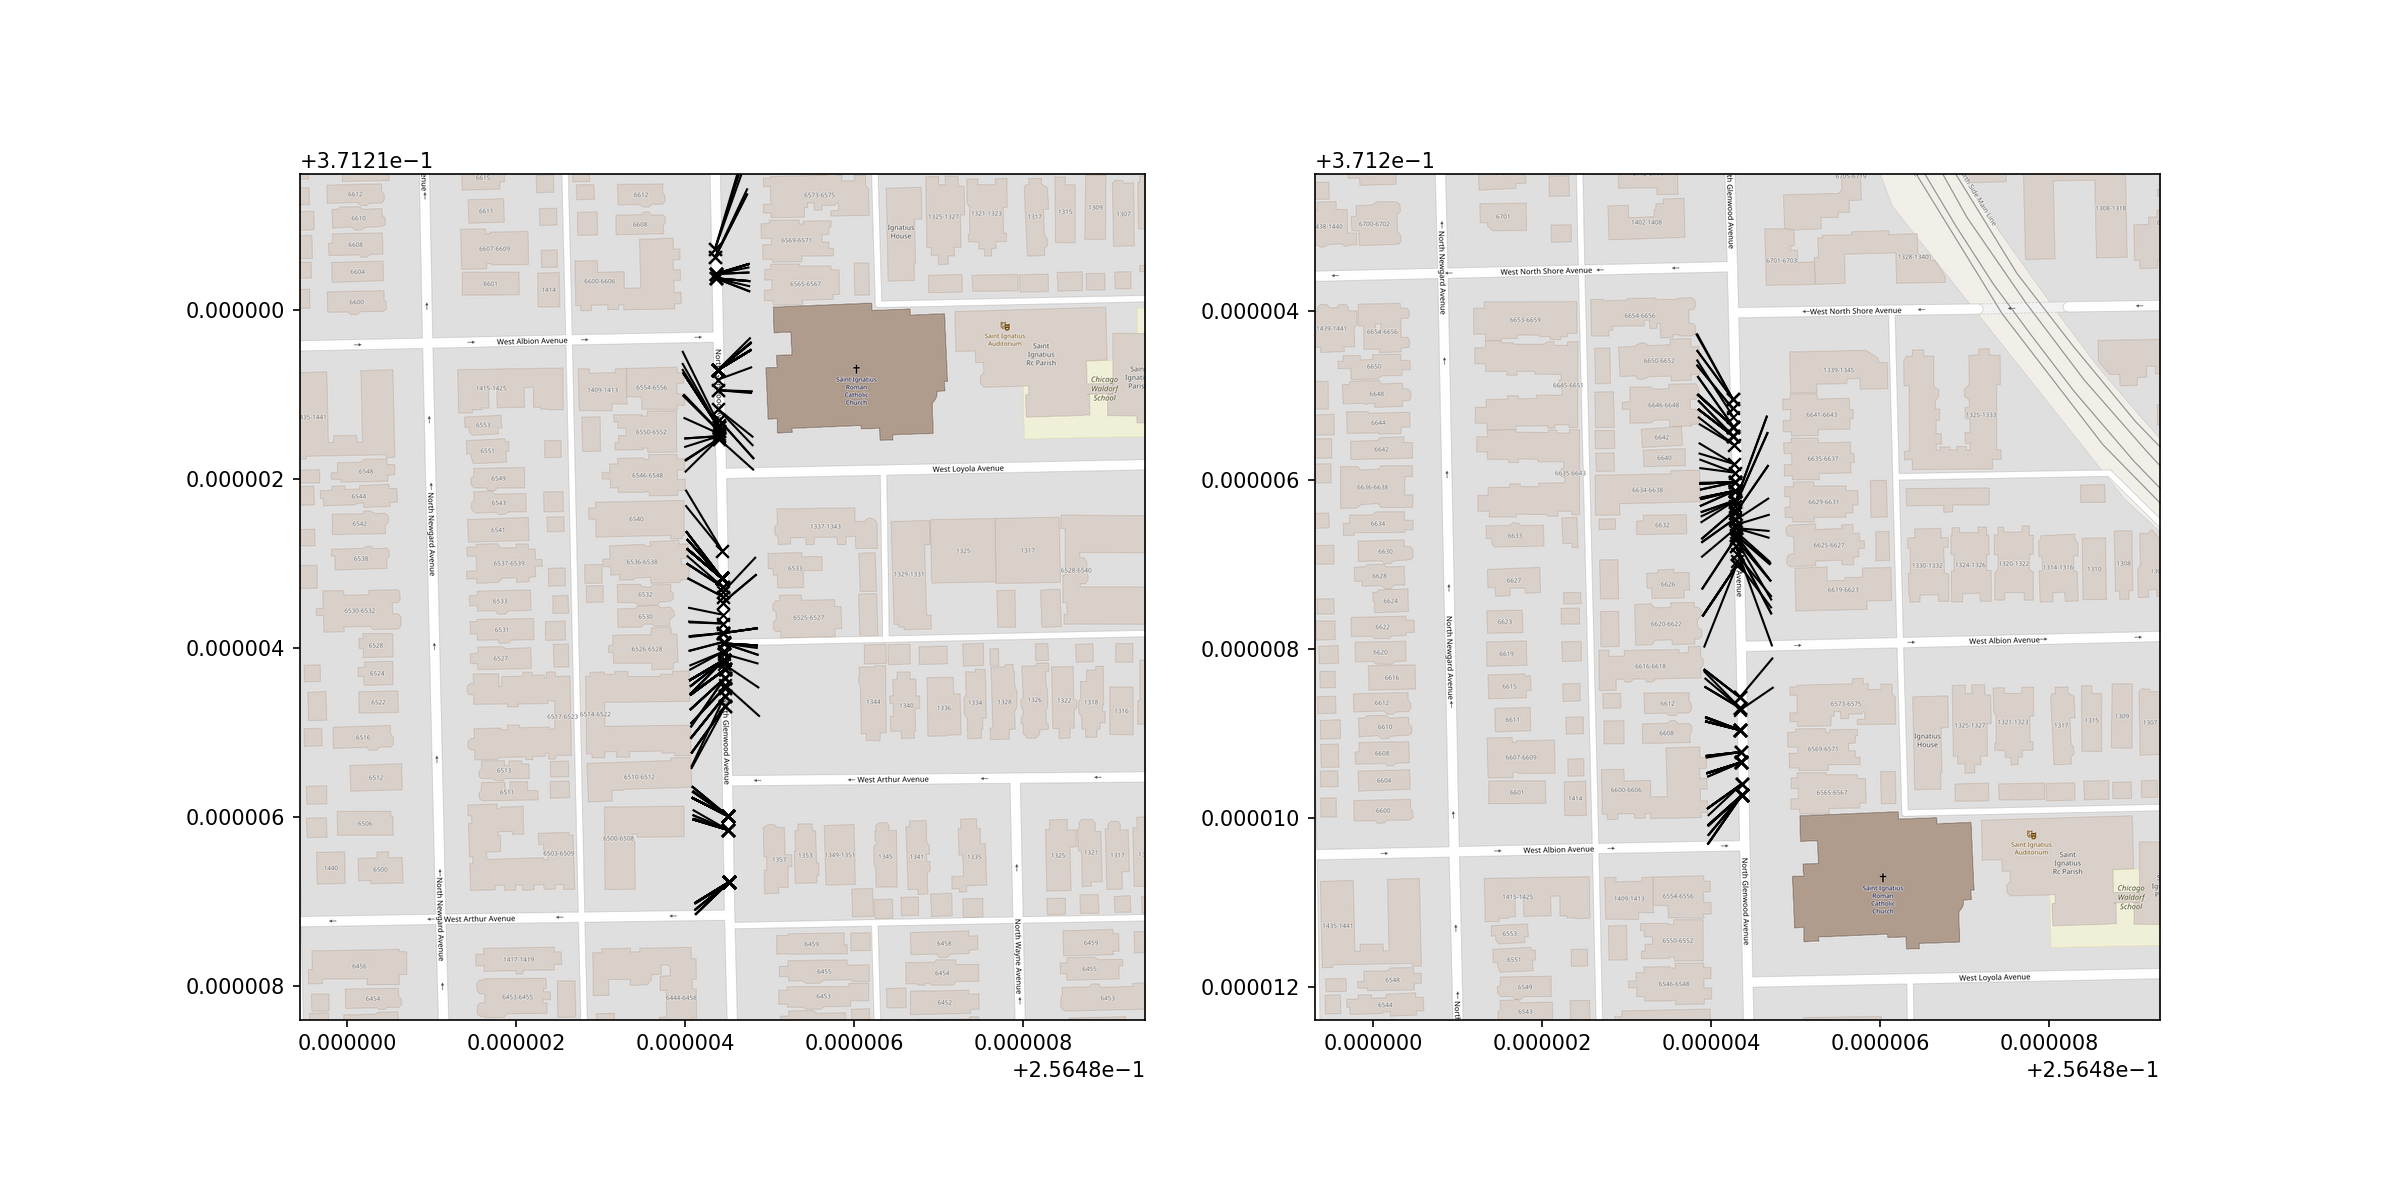
\includegraphics[width=\textwidth]{Chicago_example2.png}
  \caption{Plots for block ``065XX N GLENWOOD AVE'' and then one block to the north,
``066XX N GLENWOOD AVE''.}
  \label{fig:four}
\end{figure*}

In the absence of further information, it is hard to be certain how the coordinates of
the events are generated.  It seems that there is a large amount of artifical random
noise-- the events always align with the street network, and appear unnaturally uniformly
distributed along the street network.  The coordinates from the ``old'' file seem to
have useful information coming from which side of the street the event appears, and
there is, perhaps, some weak correlation between actual place and the coordinate.
Unfortunately, the only dataset currently available is the ``new'' file, which has
been further projected onto the street network, and ``clustered''.


\subsection{Linking with the street network}\label{sec:link_st_net}

Above, we saw a visual link between the coordinates of events and the street network.
To explore this more, we looked at the TIGER/Lines\regsym data, specifically the
``Roads'' and ``Edges'' collections.

The ``Roads'' collection gives lines on a map, each representing a long stretch of
a named road (for example, many blocks).  Sometimes a road may have two or more names
or identities, and here the line can appear twice with different metadata.

The ``Edges'' collection gives lines on a map, each a short section of road (say,
between two intersections).  Each line is unique.  There is some address information,
for example, giving the start and end numbering for the left and right side of the
street.  However, we have found that this is rather inconsistent, and there are many
sections of roads without address information while e.g. OpenStreetMap shows buildings.

There is superficially an extremely close match between the location of events from
the crime data, and the TIGER/Lines\regsym edge data.
\begin{itemize}
\item We have found it very
useful to remove from the ``Edges'' collection streets that have no name (which are
typically back-alleyways etc.) or streets with names which are obviously not roads,
such as ``ALLEY''.  We call this the ``reduced street network''.
\item For each crime event location, we project this to the street network (find the
closest point on the street network).
\item We compare the ``block'' name with the name(s) from the TIGER/Lines\regsym data.
\item There is \emph{generally} an extremely good match, including street numbering
  information if this is available.
\end{itemize}
However, from an \emph{algorithmic} point of view, we find a number of problems.
\begin{itemize}
\item Any number of minor spelling differences, which are hard to automatically correct.
\item A sizable number of outliers, where events just appear to be geocoded incorrectly.
\item Some surprising ``systematic'' errors, of the form of an event being geocoded to
  e.g. the 5900 block of North Cicero Avenue but having the ``block'' name of
  ``059XX S CICERO AVE''.  We are genuinely puzzled by this error, as while it would seem
  easy for a human to confuse North and South, we would have expected the coordinates
  to be geocoded from the address; or the address looked up from some coordinates.  It is hard
  to see how they could get out of synchronisation.
\item A few cases where the geometry fails: e.g. an event very close to an intersection,
  where the street it is closest to is the ``wrong'' one.
\end{itemize}

The pattern (in the ``new'' data) seen in the left plot of Figure~\ref{fig:three} is very
common: namely that events are ``clustered'' towards the middle of a street ``segment''.
Here ``segment'' seems to be the continuous part of a street between two intersections.
However, it is not entirely systematic as to what counts as an ``intersection''.
Often we must work with the reduced street network (i.e. ignore alleyways etc.) but the
case of ``054XX S LAFLIN ST'' is confusing here, as we see two clusters, but on the
streets to the east and west, we only have one cluster (despite, in all cases, there
being minor roads forming intersections.)


\subsection{Street data specific to Chicago}

The Chicago Data Portal also provides a shapefile of the street network, \cite{cstreets}.
This data is rather similar to, but not identical to, the reduced street network.
When comparing the resulting network with the crime events, we find exactly the same
problems as before.  Further details are in a Jupyter Notebook.

\subsection{Using open address data}

A large database of building-level address data (for the USA) is available from
\cite{oa}.  This appears to be very similar to the sort of building level address
data which one could extract from OpenStreetMap, for example.  We explored trying to
match each ``block'' in the crime event collection with building addresses.  This
suffers from similar problems as we encounted above, namely minor spelling errors,
and incorrect data.  Here we also find that a street name and number may not be
unique, and so some clustering was necessary.  The major problem, however, is that
not every ``block'' actually contains a building.

In summary then, it seems possible that a concerted effort could come up with some
automatic way to assign (most, or nearly all) crime event locations to a segment or
section of the street network (or perhaps, maybe limited to property crime, a group
of candidate buildings).  It does seem, however, that a considerable amount of effort
would be required.  We revisit these ideas in Section~\ref{sec:sf_assign_to_buildings} below.




\section{San Francisco data}

This data is from \cite{sfdata} and again is regularly updated.  This study uses data
covering 1st January 2003 to 13th September 2017, inclusive.
There appears to be very
little detail as to the meaning of the fields.  Some sample plots, Figure~\ref{fig:two},
shows that the locations are much more highly clustered than the Chicago data.

\begin{figure*}
  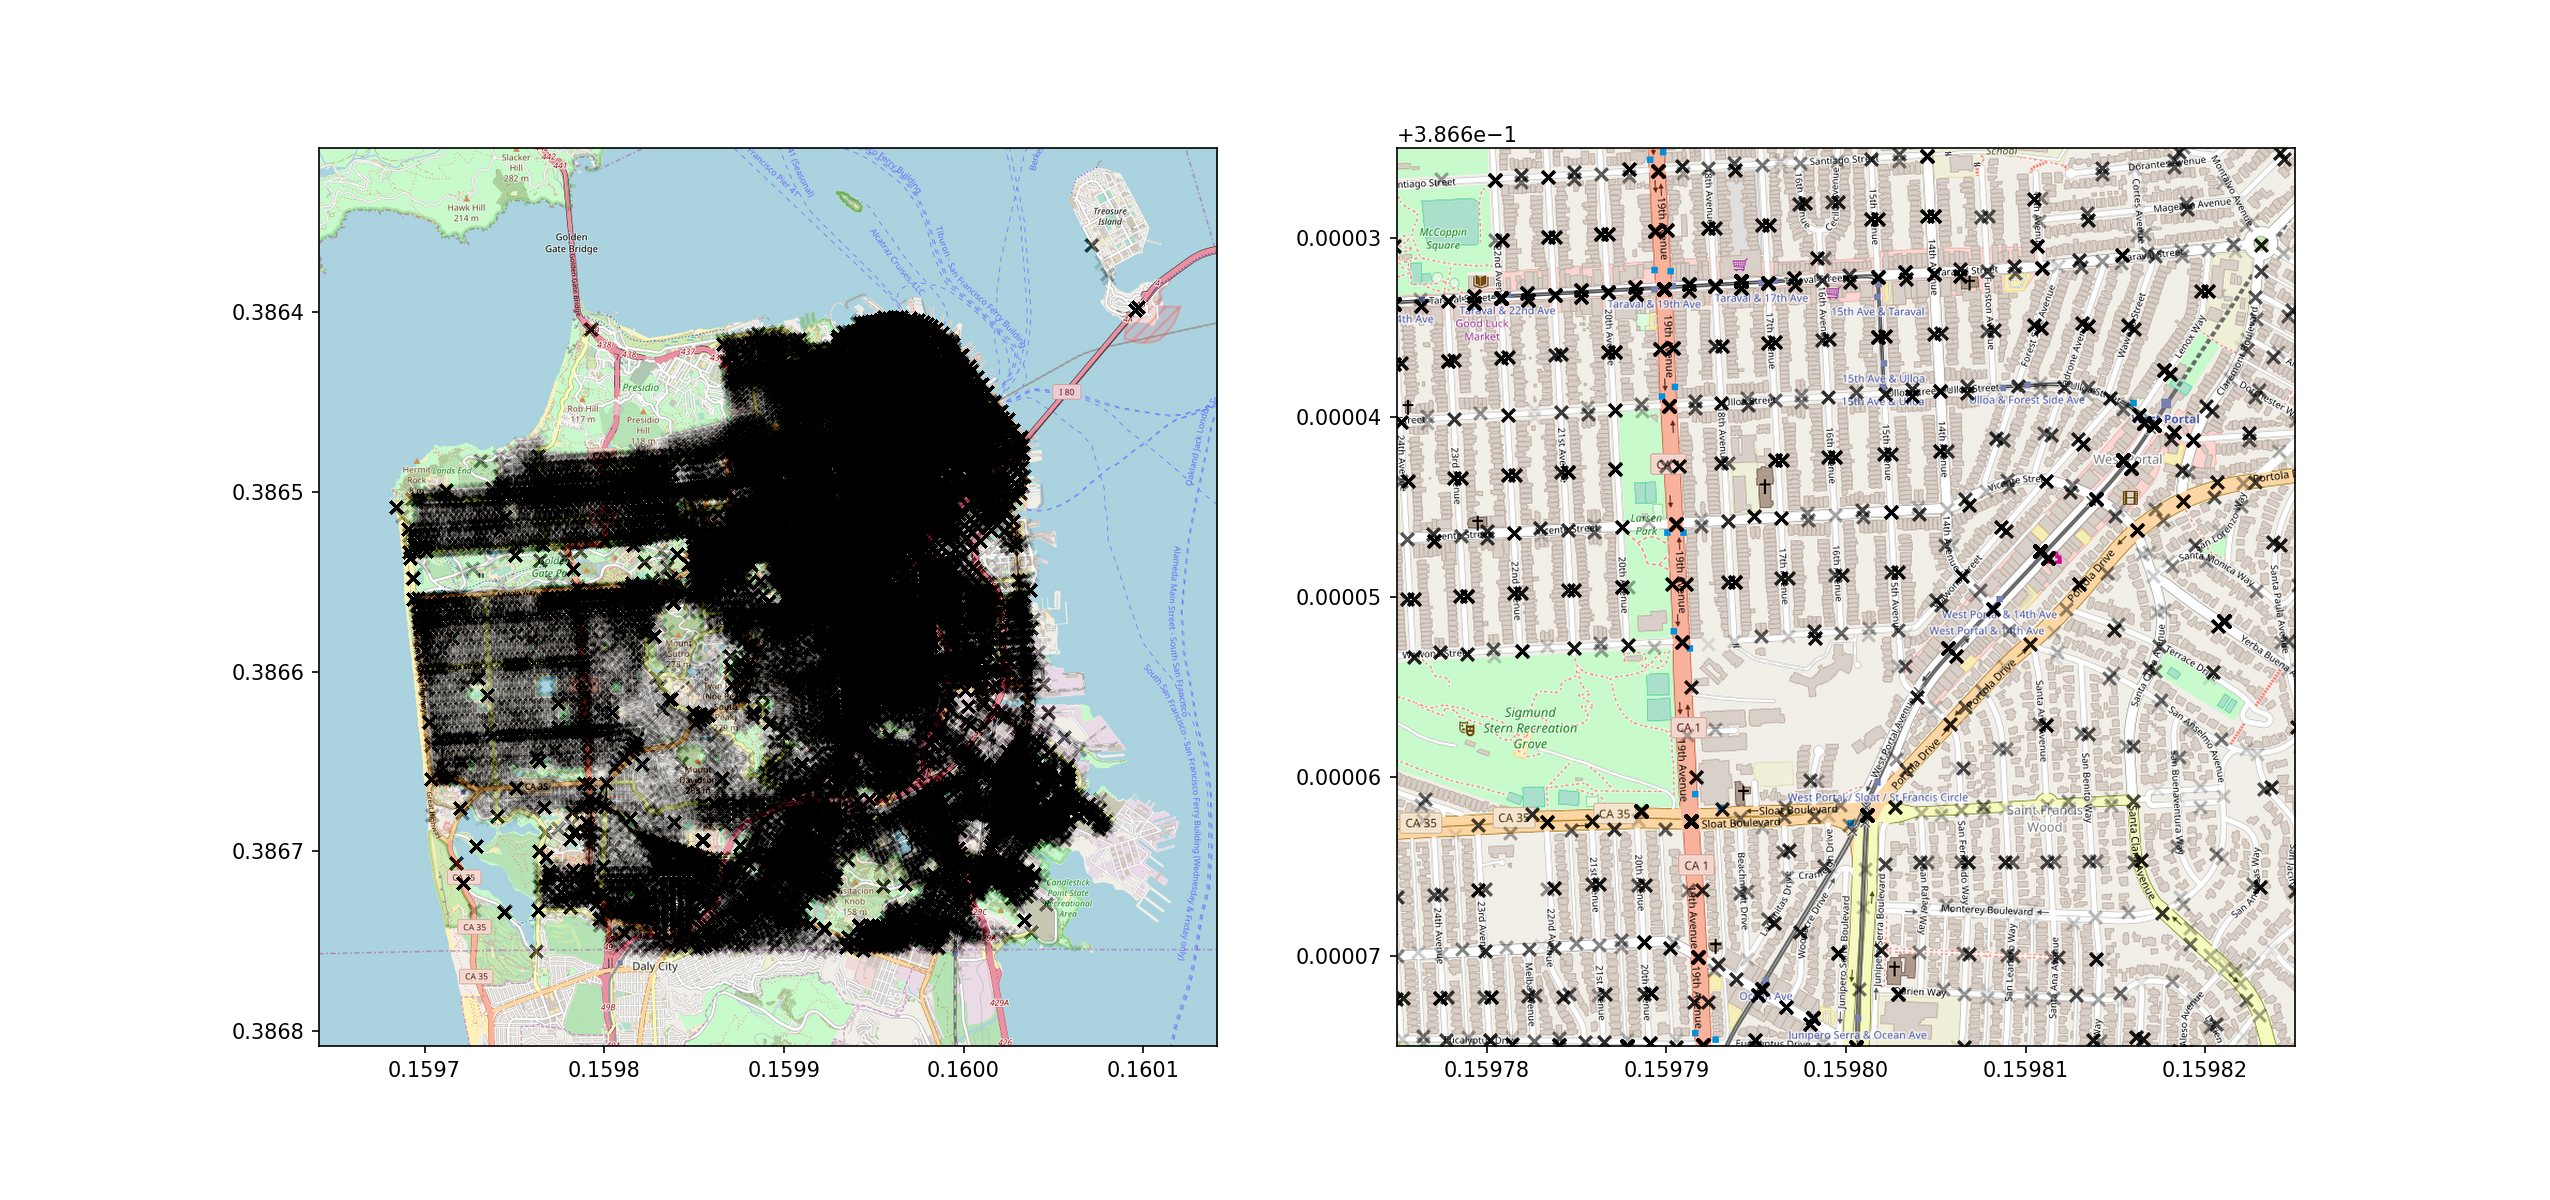
\includegraphics[width=\textwidth]{SF_overview.png}
  \caption{The complete San Francisco dataset, and an extract showing a typical ``clustering'' of events.}
  \label{fig:two}
\end{figure*}

The data comes as a CSV file, from which we find the following meanings for the fields:
\begin{itemize}
\item \texttt{PdId}, a unique identifier for each row.
\item \texttt{IncidntNum}, seems to be unique to the \emph{incident} but there may be multiple
  rows with the same number.  The \emph{vast} majority of repeats are multiple offences committed at the same time
  and place.  A rather small number are linked crimes across different times (often e.g. a stolen vehicle
  which is later recovered).
\item \texttt{Category}, which is the crime type, from 39 options, e.g. ``BURGLARY''.
\item \texttt{Descript}, a ``sub type'' of crime, to be linked with \texttt{Category}.
  Seems to be detailed; for example, ``BURGLARY'' is associated with 57 sub-types, for example
  ``BURGLARY OF STORE, ATTEMPTED FORCIBLE ENTRY''.  This form is typical, combining a location
  description with an MO.
\item \texttt{DayOfWeek}, \texttt{Date} and \texttt{Time} which combine to give the timestamp
\item \texttt{PdDistrict}, which is one of a small number of district names, e.g. ``TENDERLOIN''.
\item \texttt{Resolution}, which is one of a small number of options, e.g. ``ARREST, BOOKED''.
\item \texttt{Address} which is always of the form ``200 Block of SAN JUAN AV'' (number rounded to
  nearest 100) or of the form ``INDIANA ST / MARIPOSA ST'' (in this case, the ordering of the
  two streets appears slightly arbitrary, and both may occur).  We will see that these latter types
  are intersections.
\item \texttt{X}, \texttt{Y} and \texttt{Location} which give the (same) Longitude and Latitude.
  A very small number of locations are false, being (90, -120.5).
\end{itemize}

The important point to note is that each crime event can appear multiple times, sometimes for
different offences, but also sometimes for the same offence.  Care should be taken to not double
count!


\subsection{Geo-coding}

We already see from Figure~\ref{fig:two} that the events seem to be much more clustered
than the Chicago data.  Again, the address field is partly anonymised.  For each unique
address, we look at all coordinates for that address.  We find three distinct patterns:
\begin{itemize}
\item Multiple coordinates, but all so close together they are, up to numerical error,
  essentially unique; or
\item Coordinates which are close, up to around 12m apart (mostly these are cases where the
  two points are different sides of the same street); or
\item A significant tail of coordinates further apart.  These seem to be a mixture of
  genuine errors, and unique addresses with multiple clusters of coordinates associated
  with them.
\end{itemize}
This is illustrated in Figure~\ref{fig:five}.

\begin{figure*}
  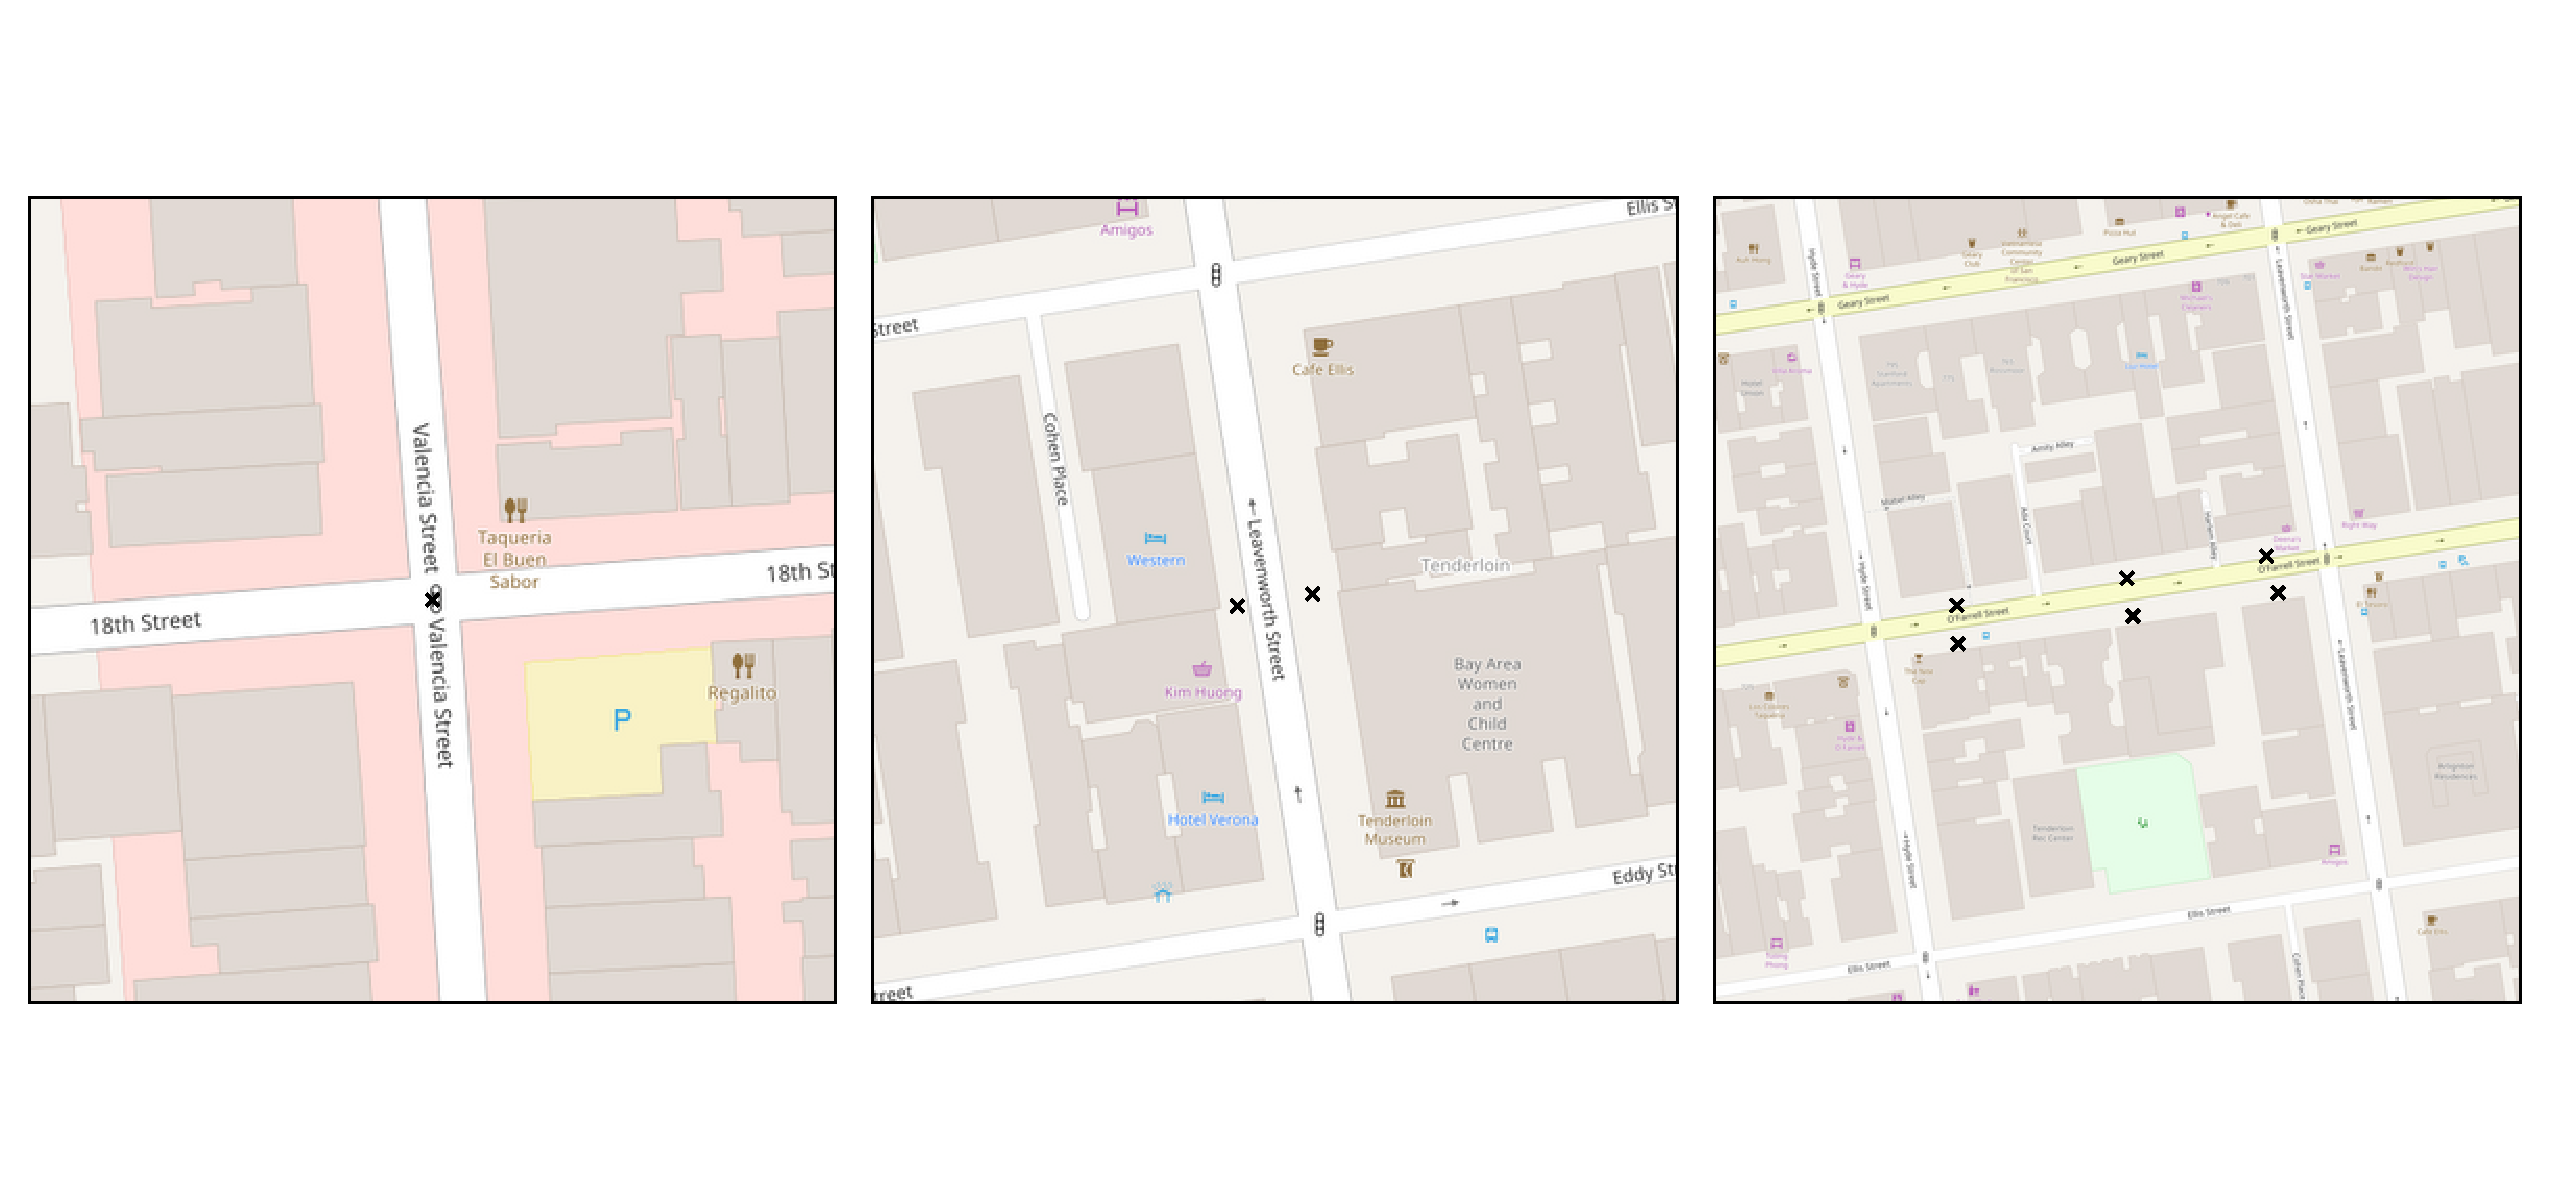
\includegraphics[width=\textwidth]{sf_types.pdf}
  \caption{The three typical distribution of points by ``Address'': a single point at an
  intersection; two points either side of a street; the same pattern repeated for a longer
  street.}
  \label{fig:five}
\end{figure*}

Unfortunately, again things are not quite this simple.  If instead we look at the ``clusters''
(i.e. points which are really close) and then look at the one or more address lines associated
with each cluster, we find a mixture of cases where there are multiple addresses:
\begin{itemize}
\item Three or more streets intersecting.  In this case, we can find some of (but maybe not all
  of) the possible pairings between the multiple streets involved.
\item The same street, just different blocks, for example ``400 Block of KIRKWOOD AV'' and
  ``700 Block of KIRKWOOD AV''.  It may be that, like the UK data, nearby locations are always
  merged together until the count of events is sufficiently large.  (In this example,
  ``400 Block of KIRKWOOD AV'' has only one event.)  This conjecture accounts for some, but
  not all, of these cases.
\item Minor spelling errors.
\item What appear to be genuine geocoding errors; for example ``2ND AV / CABRILLO ST''
  gets confused with ``22ND AV / CABRILLO ST''.  Notice that this example reminds us of the
  Chicago data, in that this error looks ``easy for a human to make'', but it is hard to
  imagine how a computer system could allow it.  Not all the errors are of this nature,
  but many do seem to be.
\item ``The Embarcadero'' (a road on the coast at the North East of San Francisco)
  gives a good example: There is a lot of overlap between the 0 and 100 blocks of the North
  and South parts of this road.
\end{itemize}

As with the Chicago data, we have looked at the TIGER/Lines\regsym street network, and
attempted to correlate this with the points.  We find similar problems with minor spelling
variation.  Also here we have the issue that for events coded to intersections, there is
no automatic, geometry based, way of deciding which street to assign the points to.
There is also San Francisco specific data available at \cite{sfgeo}, but this appears to
be extremely similar to the TIGER/Lines\regsym data, and is sometimes less complete.

This leaves us in a situation which is similar to the Chicago data: do we trust the
``Address'' field, or the geocoding, more?  There is evidently a lot of correlation between
the two, but also a lot of conflict.






\section{Dallas}

This data is from \cite{ddata} and again is regularly updated.  This study uses data
covering June 2014 to 7th December 2017.  As we shall see, assigning exact
times to events can be difficult!  There appears to be very
little detail as to the meaning of the fields.  Some sample plots, Figure~\ref{fig:dallas},
shows that the locations are much more distributed than in either of the other two examples.

\begin{figure*}
  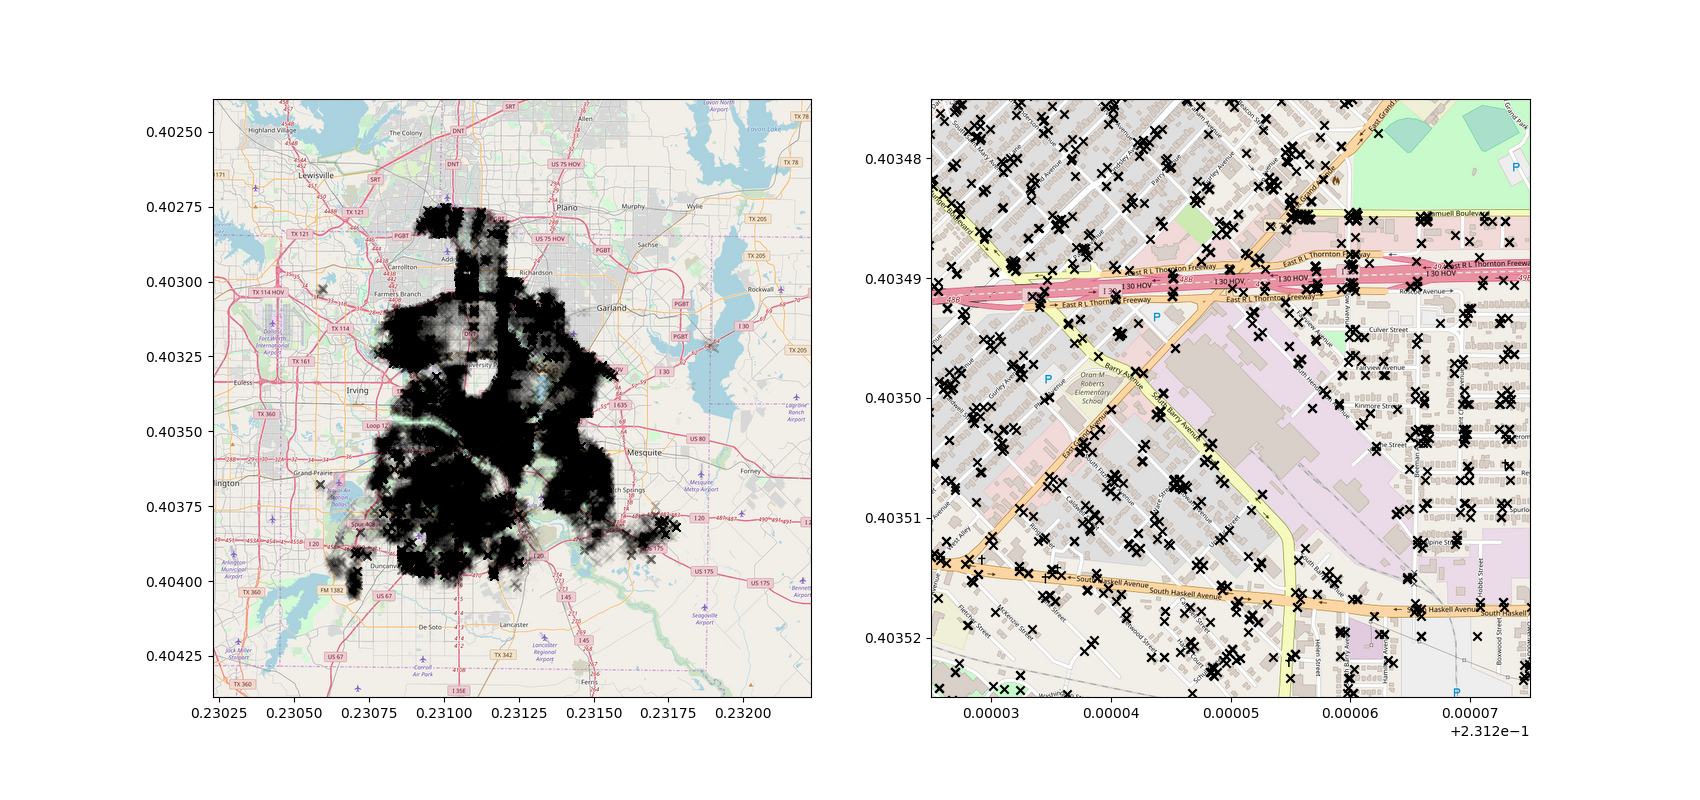
\includegraphics[width=\textwidth]{Dallas_overview.png}
  \caption{The complete Dallas dataset.}
  \label{fig:dallas}
\end{figure*}

The dataset is extraordinarily rich, and amazingly includes detailed information about the victim
of many crimes!  We shall ignore this information, and just look at crime type, timestamp, and
location information.  Each row has an incident number, but many rows share the same number.
Upon close examination, this is because multiple ``events'' are coded for the same crime.  For example,
one row of the data may detail the victim of the crime, and then other rows will detail witnesses
to the crime.  It appears that the crime type and location does not change, so to correctly
process the data, it is merely necessary to not double count.  Our library code handles
this automatically.

There is a lot of timestamp related information, but mostly these are duplicates.  Each row has a
``start'' and ``end'' time (which may be in the ``wrong'' order!)  There is also timestamp information
about when the call for service was recieved.  There is unfortunately a (very) large amount of noise
in this data, and no simple relationship between the start, end and call times.  Our library extracts all
three timestamps.

Address information is similarly reported multiple ways, but our investigation
suggests that the separated fields here give the most accurate address.  Remarkably, completely accurate
addresses (and not just the ``block'') are given.

We extract the following fields:
\begin{itemize}
\item \texttt{Service Number ID}, \texttt{UCR Offense Description} and \texttt{UCR Offense Name}
  which give the identification of the crime, the crime type, and some minimal amount of extra information.
\item \texttt{Starting  Date/Time}, \texttt{Ending Date/Time} and \texttt{Call Date Time} which we presume
  are the probable start and end times of the crime, and the time of the 911 call for service.  A tiny number
  of records are missing data.  In principle, this would allow us to use \emph{Aoristic analysis}, \cite{ratcliffe}.
  Unfortunately, there appears to be no simple way to interpret these numbers.  Figure~\ref{fig:dallas_times}
  shows the distribution in time gaps.  22\% of records have the same start and end times, and 29\% have
  a time gap of at most 5 minutes.  However, as the figure indicates, a significant number of events have a time
  gap of over a day, and some of over a week.  Similarly, there can be a huge difference in time between
  the ``call'' time and the end time.
\item \texttt{Incident Address}, \texttt{City} and \texttt{Zip Code} giving the address.  This appears to
  be accurate, not obscured to the nearest block (for example).  The vast majority of records have an address.
\item \texttt{Location1} which gives longitude and latitude coordinates, but appears to always be empty for
  events after around the beginning for 2017, or before mid 2015.
\item \texttt{X Coordinate} and \texttt{Y Coordinate} give projected coordinates.  Most, but not all,
  records have these.
\end{itemize}

\begin{figure*}
  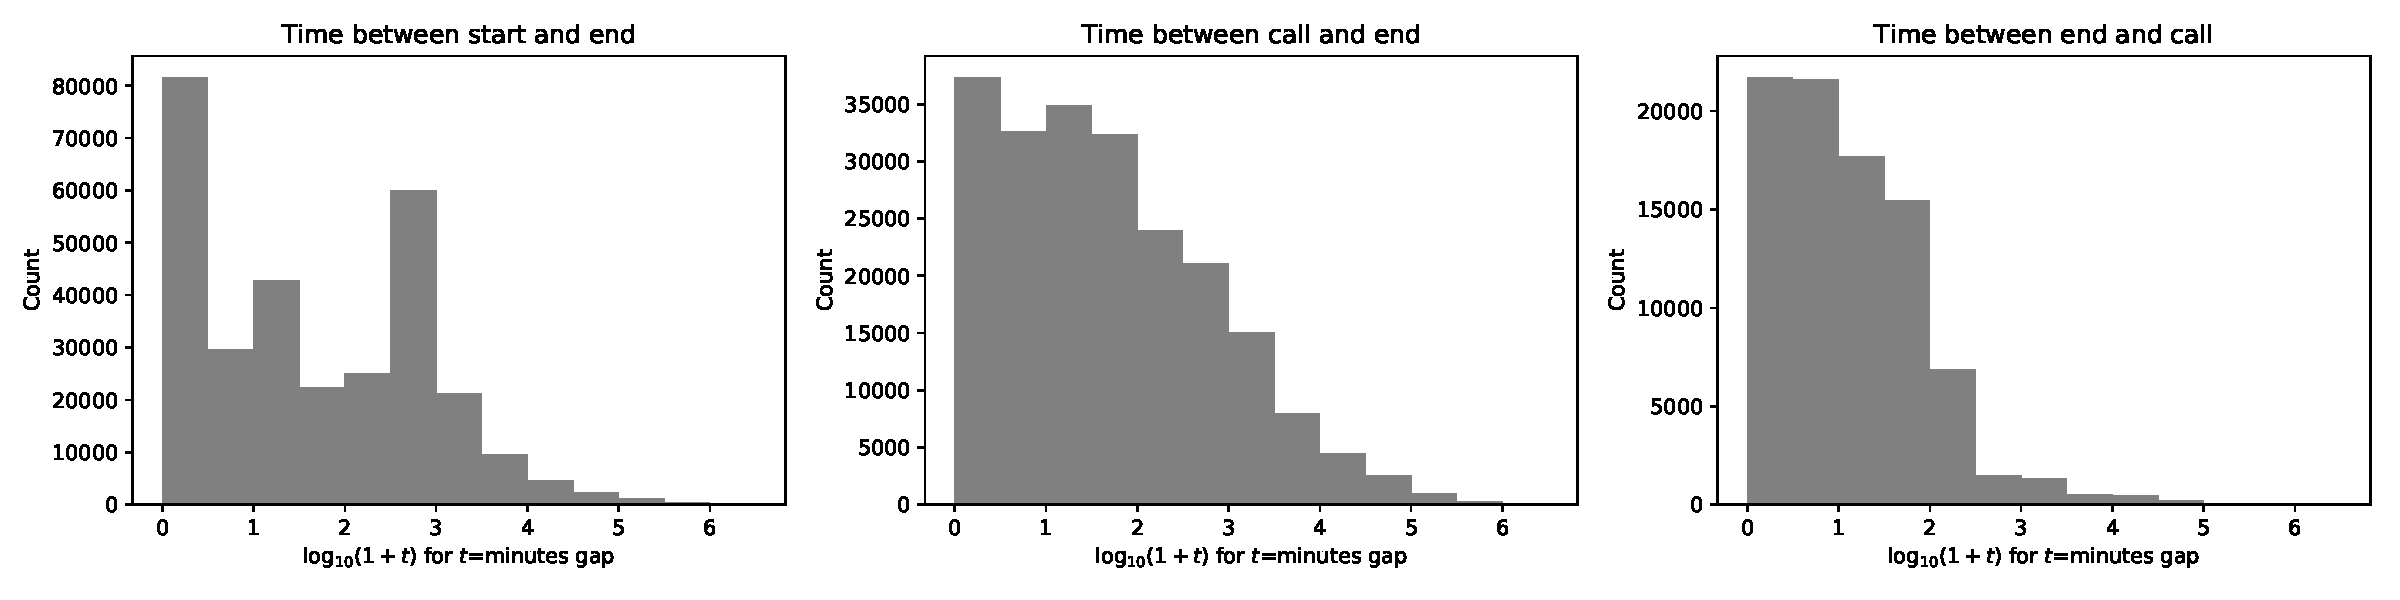
\includegraphics[width=\textwidth]{dallas_times.pdf}
  \caption{From left to right: The time gap between the ``start'' and ``end'' timestamps;
  the time gap between the ``call'' and ``end'' timestamps (if positive);
  the time gap between the ``end'' and ``call'' timestamps (if positive).}
  \label{fig:dallas_times}
\end{figure*}



\subsection{Geo-coding}

For some records, those from 2016 and late 2015 it seems, we have two sources of geo-coding.  It appears that
EPSG:2845 is used to project the longitude and latitude coordinates, but there is not an exact match
between the two geocodings.  Figure~\ref{fig:dallas_geocoding} shows the two geocodings.  By
carefully examining a basemap, it appears that (with a few outliers) the longitude and latitude
are always in the centre of the street, exactly outside the correct address.  The projected coordinates
seem reasonably randomly offset; we have not been able to see much pattern in the difference, except
that the lines connecting the two points are often aligned with the direction of the street (the
pattern is similar to the relation between the ``old'' and ``new'' geocodings for the Chicago data).

\begin{figure*}
  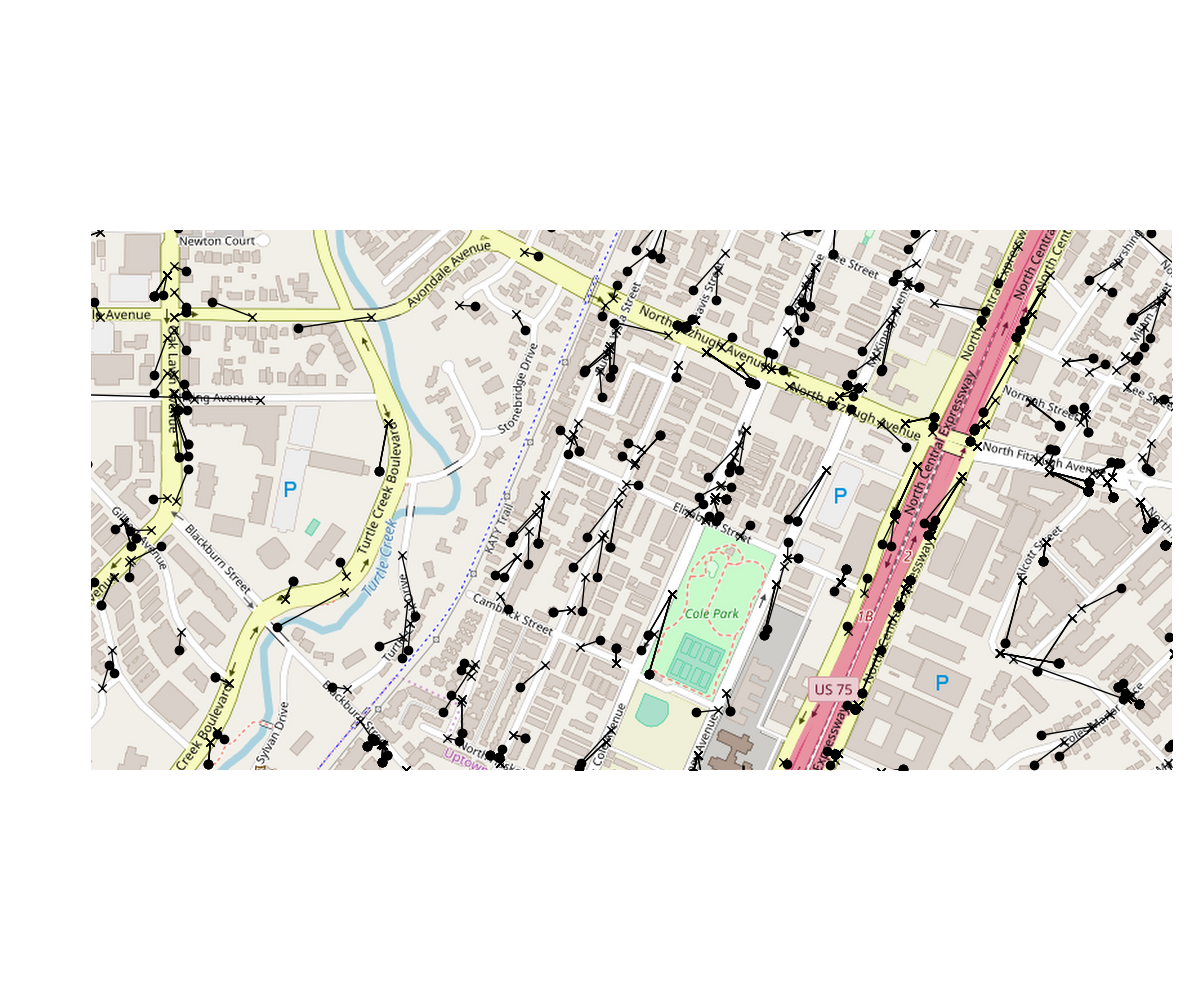
\includegraphics[width=\textwidth]{dallas_geocoding_1.png}
  \caption{Extract of the Dallas data, with event locations plotted.  A $\times$ marks the longitude
and latitude, while $\bullet$ marks the projected x,y coordinates, and a line joins the locations.}
  \label{fig:dallas_geocoding}
\end{figure*}

We would almost certainly prefer to use the longitude and latitude coordinates, but these are only
provided for a subset of the records.

There is also a street centre-lines file available a \cite{dstreets} which yet again is similar
to, but not quite identical, to the TIGER/Lines\regsym data.  We note that the Dallas city
limits straddle two TIGER/Lines\regsym files, and so the data from \cite{dstreets} is easier to use.



\section{Local reassignment of coordinates}\label{sec:reassign}

For a variety of reasons, we have seen that while all three datasets purport to give
exact event coordinates, we do not believe that the coordinates are accurate, beyond
that they do appear on, or close to, the correct ``block'' of the street the event
occurred on.  (Which itself may be far from the actual event location, if that
event occurred in a park, or in an alleyway, for example).

Is this necessarily a problem?  If we are aggregating the data up to even quite a small
areal unit, and certainly if we are looking at larger areas, such as community
neighbourhoods, police districts, etc., then clearly the exact location is unimportant.

However, we are interested in crime prediction algorithms.  These typically function
on small to very small \emph{grid} cells, or directly on the street network, see
\cite{arc, bjp, rand, rosser_sepp, rosser_nw}.
If the grid size is small, comparable to the length of a city block, then with the
clustering of events which we see, minor variation in the exact alignment of
grid cells could have a large effect, as all at once a large number of events move
across the boundaries of the cells; compare Section~\ref{sec:preds_grid} below.

For network based predictions, it perhaps becomes slightly less important for
e.g. the Chicago data, as this already appears to be aligned to the network.
However, this is artificial, and for events which occurred, in reality, close
to an intersection, it may be that the event is more naturally assigned to a
neighbouring edge in the street network.  For e.g. the San Francisco data, we
have a decision to make as which edge all the points from every intersection
belong to.

Finally, if we are interested in the performance of our algorithms on real-world data
which does have exact geocoding (e.g. internal Police data) then it would be hugely
useful to have open data which had the same characteristics.

In the subsequent sections, we develop a number of algorithms which seek to
move coordinates of events in ways which are consistent with what we have learnt above.



\section{Voroni cells for San Francisco}

The San Francisco data is hugely clustered, and we can make a very plausible conjecture
that the way the geocoding is arrived at is that cluster locations are chosen (intersections,
either side of the road, with longer roads being split up) and then the real location
is assigned to the closest cluster location.

We obviously cannot undo this procedure, but we can simulate plausible locations.
This is related, by analogy, to the general idea of ``imputation'' in statistics, where we
seek to replace missing values in data.

If we believe exactly the ``closest point'' hypothesis, then the notion of a Voronoi
(also Dirichlet or Thiessen) diagram becomes immediately important;
for an exhaustive guide, see \cite{obs}.
Given a collection $S$
of points in the plane, the ``voroni cell'' around a point $x$ is the collection of points
in the plane which are closer to $x$ than to any other member of $S$.  Voroni cells are (open)
polygons, and there are fast algorithms to compute the boundaries between cells.  We use
the algorithm implemented in \texttt{scipy} together with some of our own code to simplify
extracting voroni cells from the data which \texttt{scipy} returns.  In particular, we handle
gracefully the ``boundary cells'' which naturally extend to infinity (given that $S$ is assumed
finite).

See Figure~\ref{fig:sf_vor_1} for an example.  Here we took the given event locations for the
San Francisco data, merged locations which were within one metre of each other, and then
constructed the voroni diagram for the merged points.  In the overview plot on the left,
we see the variation in cell size: in dense housing, cells are small, but over parkland, they
become much larger.  The right plot shows clearly the polygonal shape of cells, and the locations
of ``clusters'' at intersections and either side of roads.

\begin{figure*}
  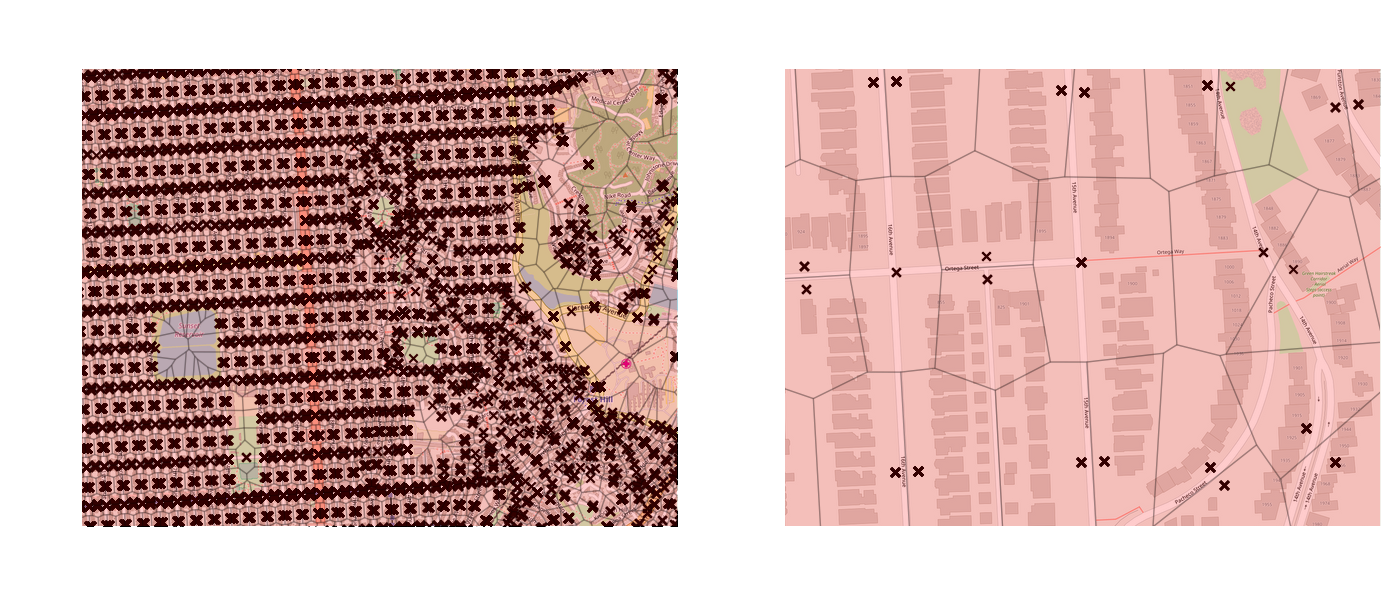
\includegraphics[width=\textwidth]{sf_vor_1.png}
  \caption{Example voroni cells for San Francisco.}
  \label{fig:sf_vor_1}
\end{figure*}

We can use this diagram to generate new locations for our events.  For each crime event,
we find the voroni cell which contains the point, and pick uniformly at random a new point
in that cell.  As cells vary in size, we constrain the new point to be within 100m of the
original point.  Figure~\ref{fig:sf_vor_2} shows the output of this process.  On the left
we show an example voroni cell, a point within it, and 200 randomly chosen points within 20m
of that point.  The plot on the right (the same basemap as Figure~\ref{fig:sf_vor_1})
shows the new locations.

\begin{figure*}
  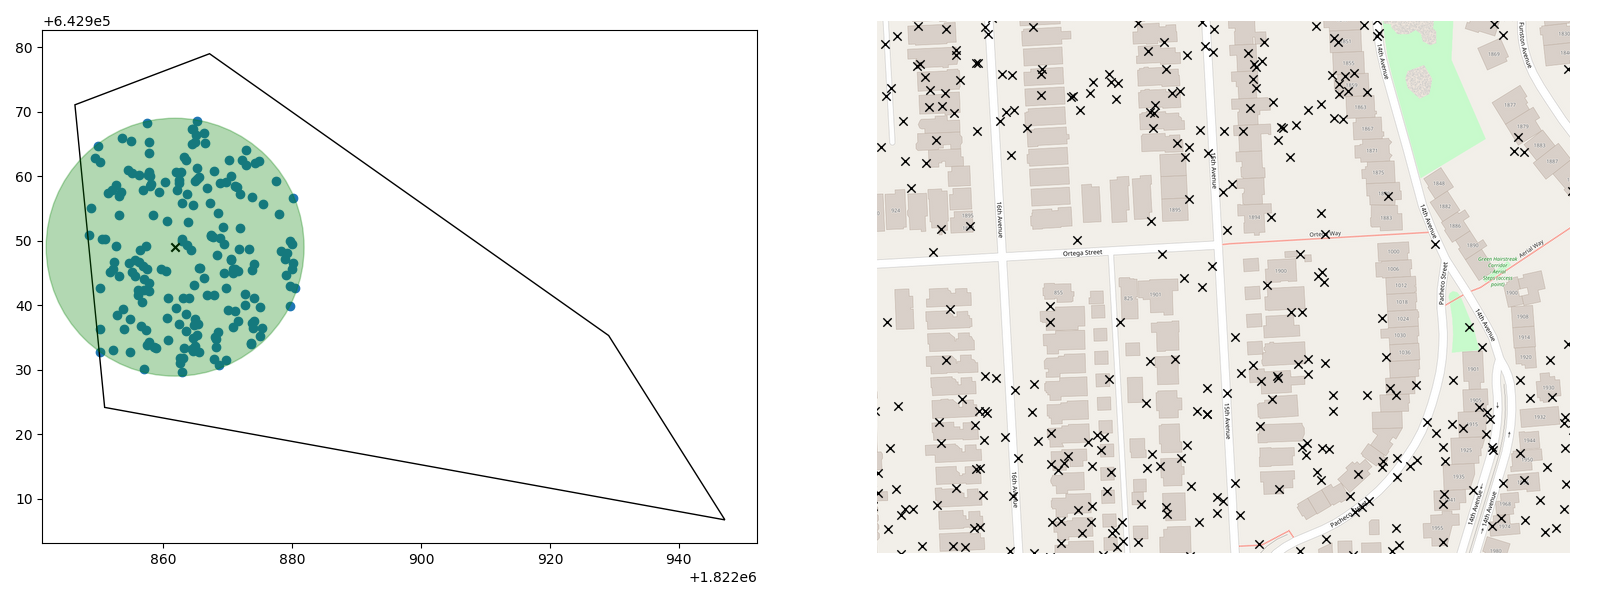
\includegraphics[width=\textwidth]{sf_vor_2.png}
  \caption{Example of using voroni cells to redistribute points.}
  \label{fig:sf_vor_2}
\end{figure*}


\subsection{Using the street network}

A variety of new crime prediction algorithms work directly on the street network, rather
than with areal grid cells, see \cite{rosser_nw, ss}.
A stated advantage of looking directly at the street network is that it is actually
physical streets which police can patrol.  From our perspective, it is also worth noting
that real-world geocoding is likely to correspond to buildings, or directly to
the street network.  Here, and below, we freely use basic ideas from graph theory, see
for example \cite{wilson}.

As the next stage of ``redistribution'', we have taken the output of the previous section,
and have projected the coordinates onto the street network (that is, choose the point on an
edge of the street network which is closest to the starting point).  For the street network, we use
the data from \cite{sfgeo}, as discussed before.  The data from \cite{tiger} seems very similar.

The result is shown in Figure~\ref{fig:sf_net_1}.  The plot on the right shows the same view
as in Figures~\ref{fig:sf_vor_1} and~\ref{fig:sf_vor_2}.  The lines join the original location
(from the input file) to the location chosen at random in the voroni cell, and then
join to the projected location.
The plot on the left just shows the projected locations.  Notice that small alleyways
are not in the street network data.  There is some ``clustering'', in fact reminiscent of
the Chicago dataset, but by comparing to the plot on the right, this seems to be caused
by an unequal number of events between those geocoded to the intersections (rather few events)
and those geocoded to the centre of the street segments (quite a few events).  As we first
redistribute uniformly in two-dimensional space, and then projected back down to the
one-dimensional street network, we see that events can end up being moved only a little way
(the bulk of events from the middle of the north/south aligned streets) but occasionally can
be moved a long way.  In the next section, we explore ways to remedy this.

\begin{figure*}
  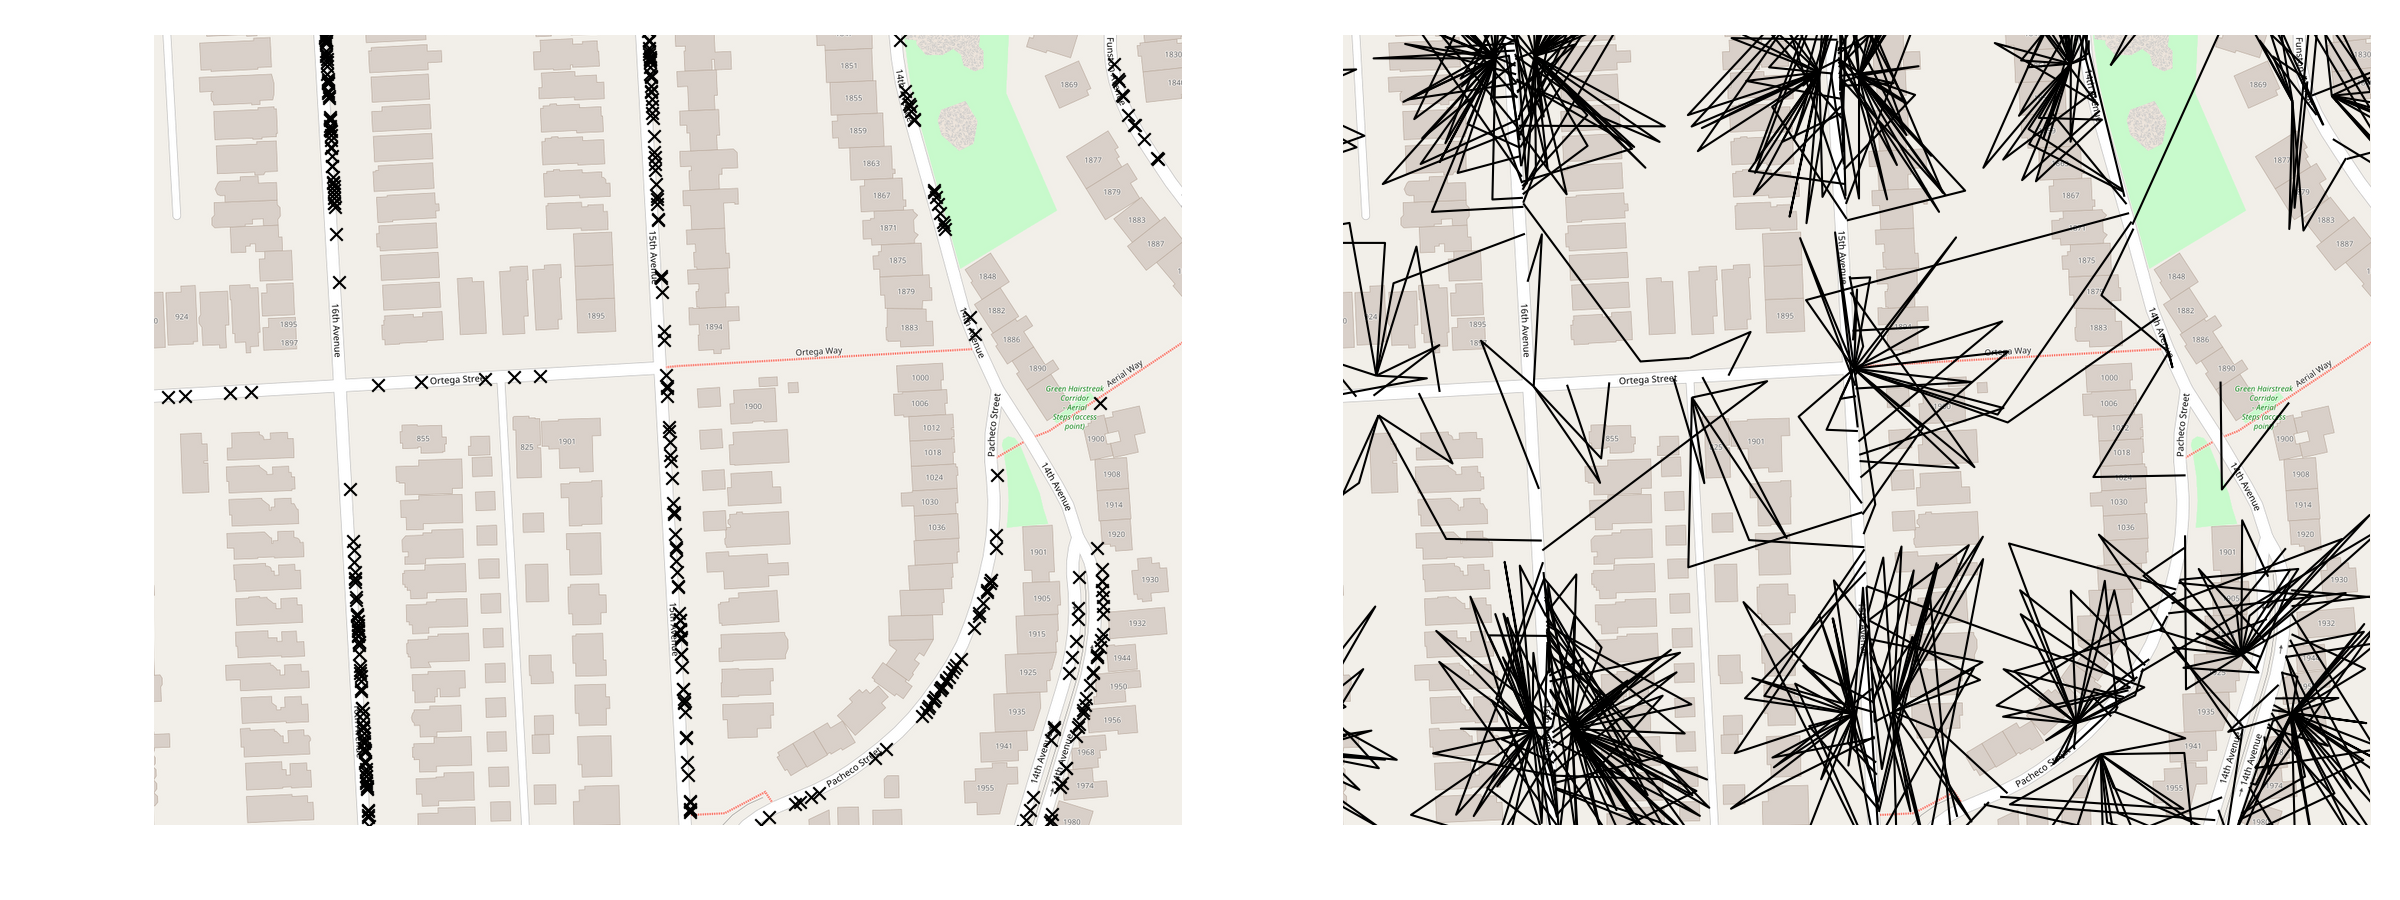
\includegraphics[width=\textwidth]{san_fran_two_stage_network_projection.png}
  \caption{Projecting the points, given by Figure~\ref{fig:sf_vor_2}, to the street network.}
  \label{fig:sf_net_1}
\end{figure*}



\subsection{Flowing points along the network}\label{sec:sf_flow}

There is a close match between the original input data and the street network.  Almost all
points fall on the network, or close to it (in the case of groupings of points either side
of a street; recall the right-hand plots in Figure~\ref{fig:five}).  There are a few outliers,
typically near parkland or the coast.

Given this, we might \emph{start} by projecting the points to the network, and then work with
an algorithm which only ``sees'' the network structure.  Again, we first aggregate very close
points, then we project to the network, and then we perform a further aggregation step on the
network, combining points which are within 10m of each other, distance now measured on the network.

The algorithm we use combines the data
of the network, and all the original input points, in the belief that the original input points
are ``close'' to the real event position.  For each input point on the network, we compute
a valid subset of the network which we may move the point to, by starting at the input point, and
traversing the network according to these rules:
\begin{itemize}
\item We can move to any location which is within a \emph{minimum} distance of start point;
here we used 50m.
\item We may only move at most a \emph{maximum} distance; we use 250m.
\item If we encounter another input point, then we will stop walking, subject to the condition
that we can continue up to the minimum distance.
\item We only consider the shortest paths when computing the ``blocking'' points in the
step above.
\end{itemize}
The idea is that we can move anywhere within the minimum distance, but we can also move
further, up to the maximum distance, so long as we don't encounter another input point.
We hence adaptively
change the size of the region we consider, according to the density of the input points.
Figure~\ref{fig:sf_flow_network} illustrates this: to the north and west we stop at the next
input point, but to the south and west we continue a little further until we reach the 50m
minimum limit.

\begin{figure}
  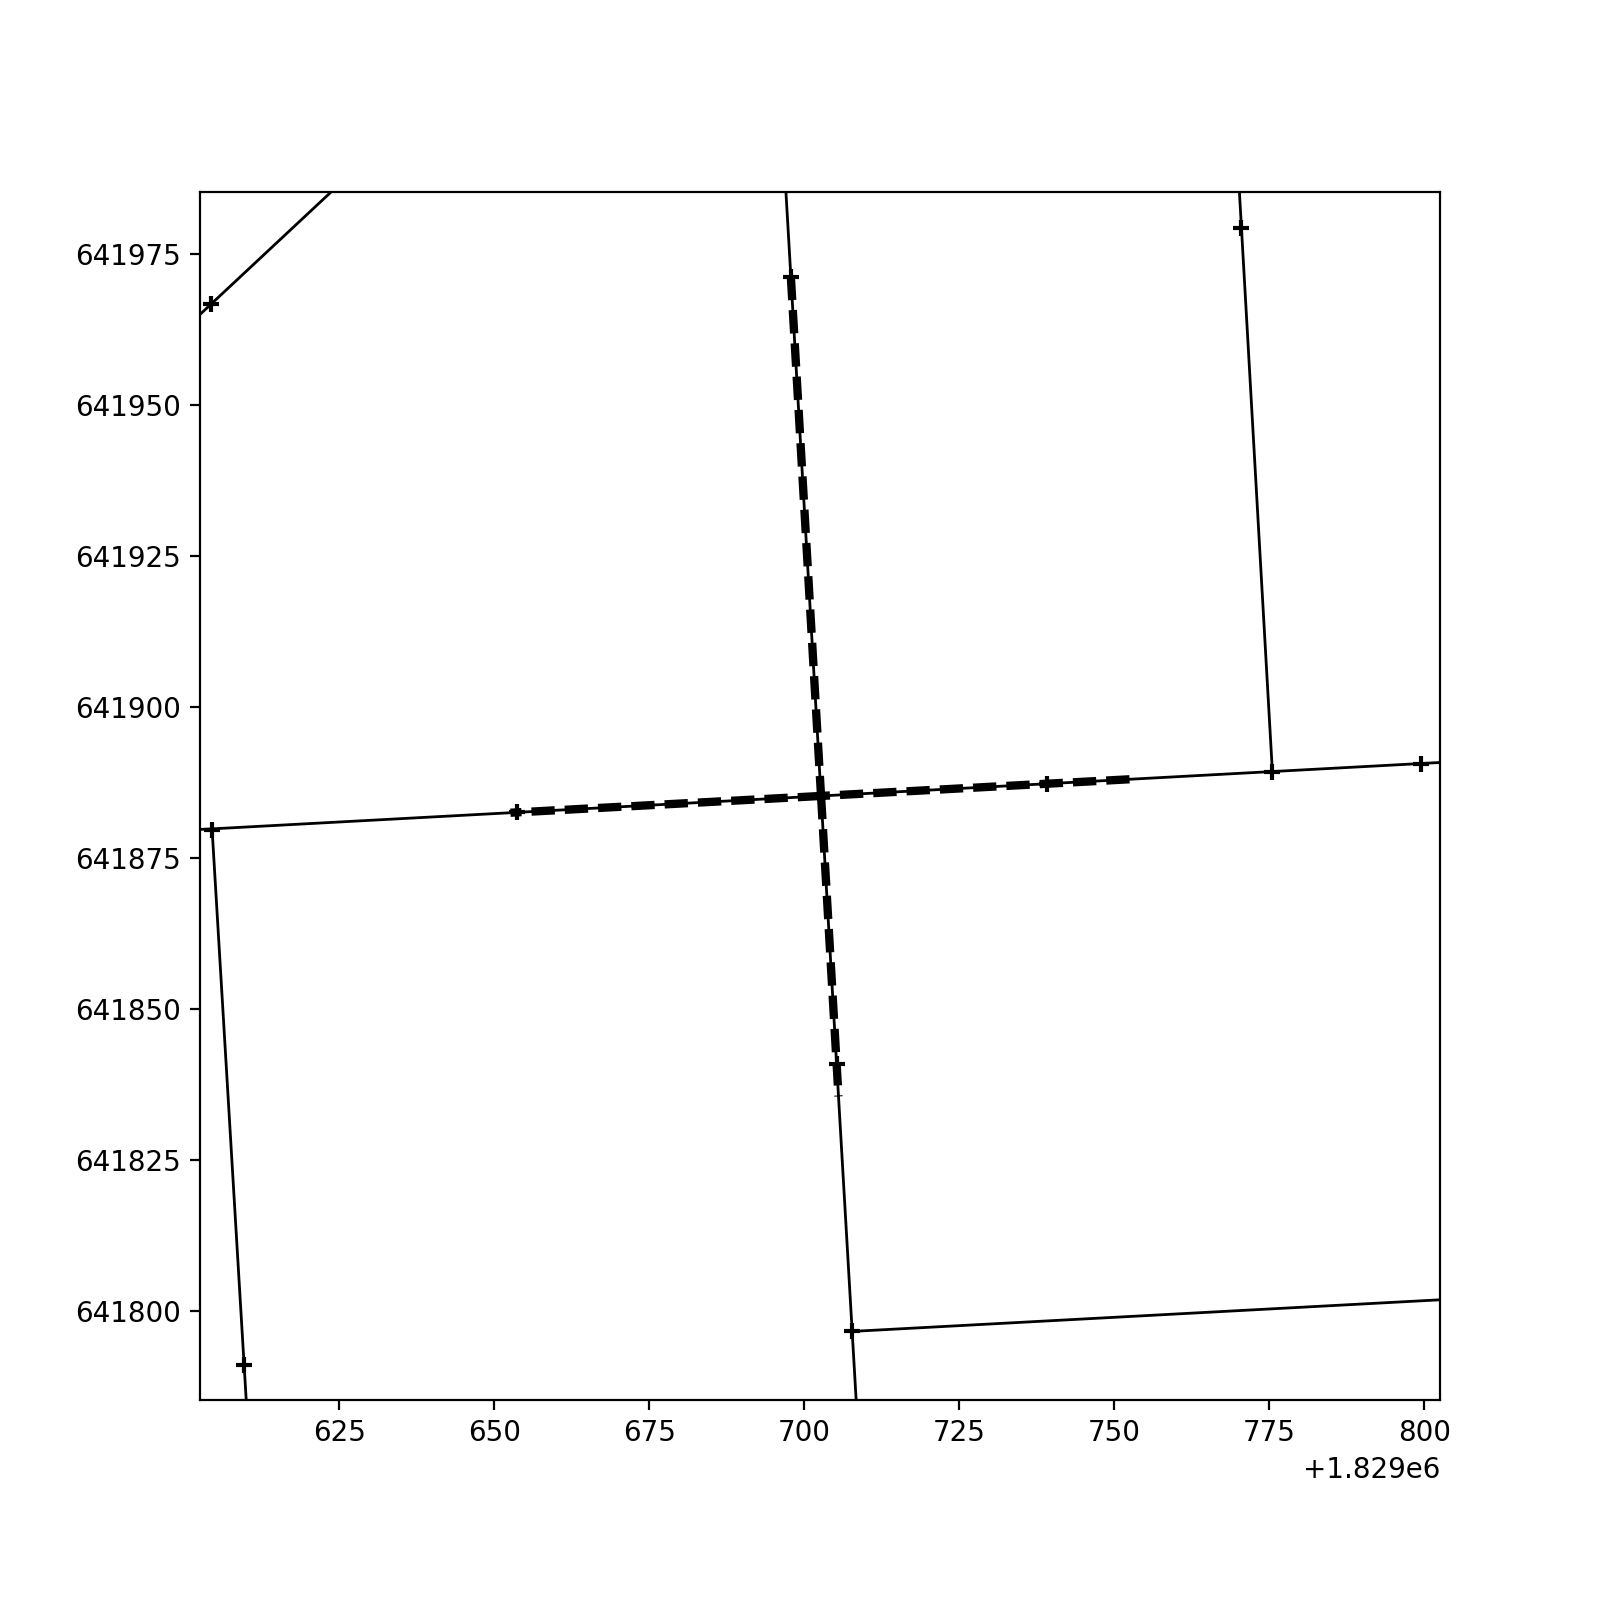
\includegraphics[width=3.5in]{sf_flow_network.png}
  \caption{The valid region we can move to from the point at the intersection.
The street network is marked with thin lines, input points by $+$ marks, and the valid
region by the thick dashed line.}
  \label{fig:sf_flow_network}
\end{figure}

Then to redistribute points, we pick uniformly at random a new point in the valid subset,
given as above.  Figure~\ref{fig:sf_flow_redist} shows the result, again for the same
basemap as in Figure~\ref{fig:sf_net_1}.  As compared to Figure~\ref{fig:sf_net_1} the
distribution of points is somewhat more uniform.  Notice that the TIGER/Lines\regsym
street network contains more streets than the San Francisco city street network.

\begin{figure*}
  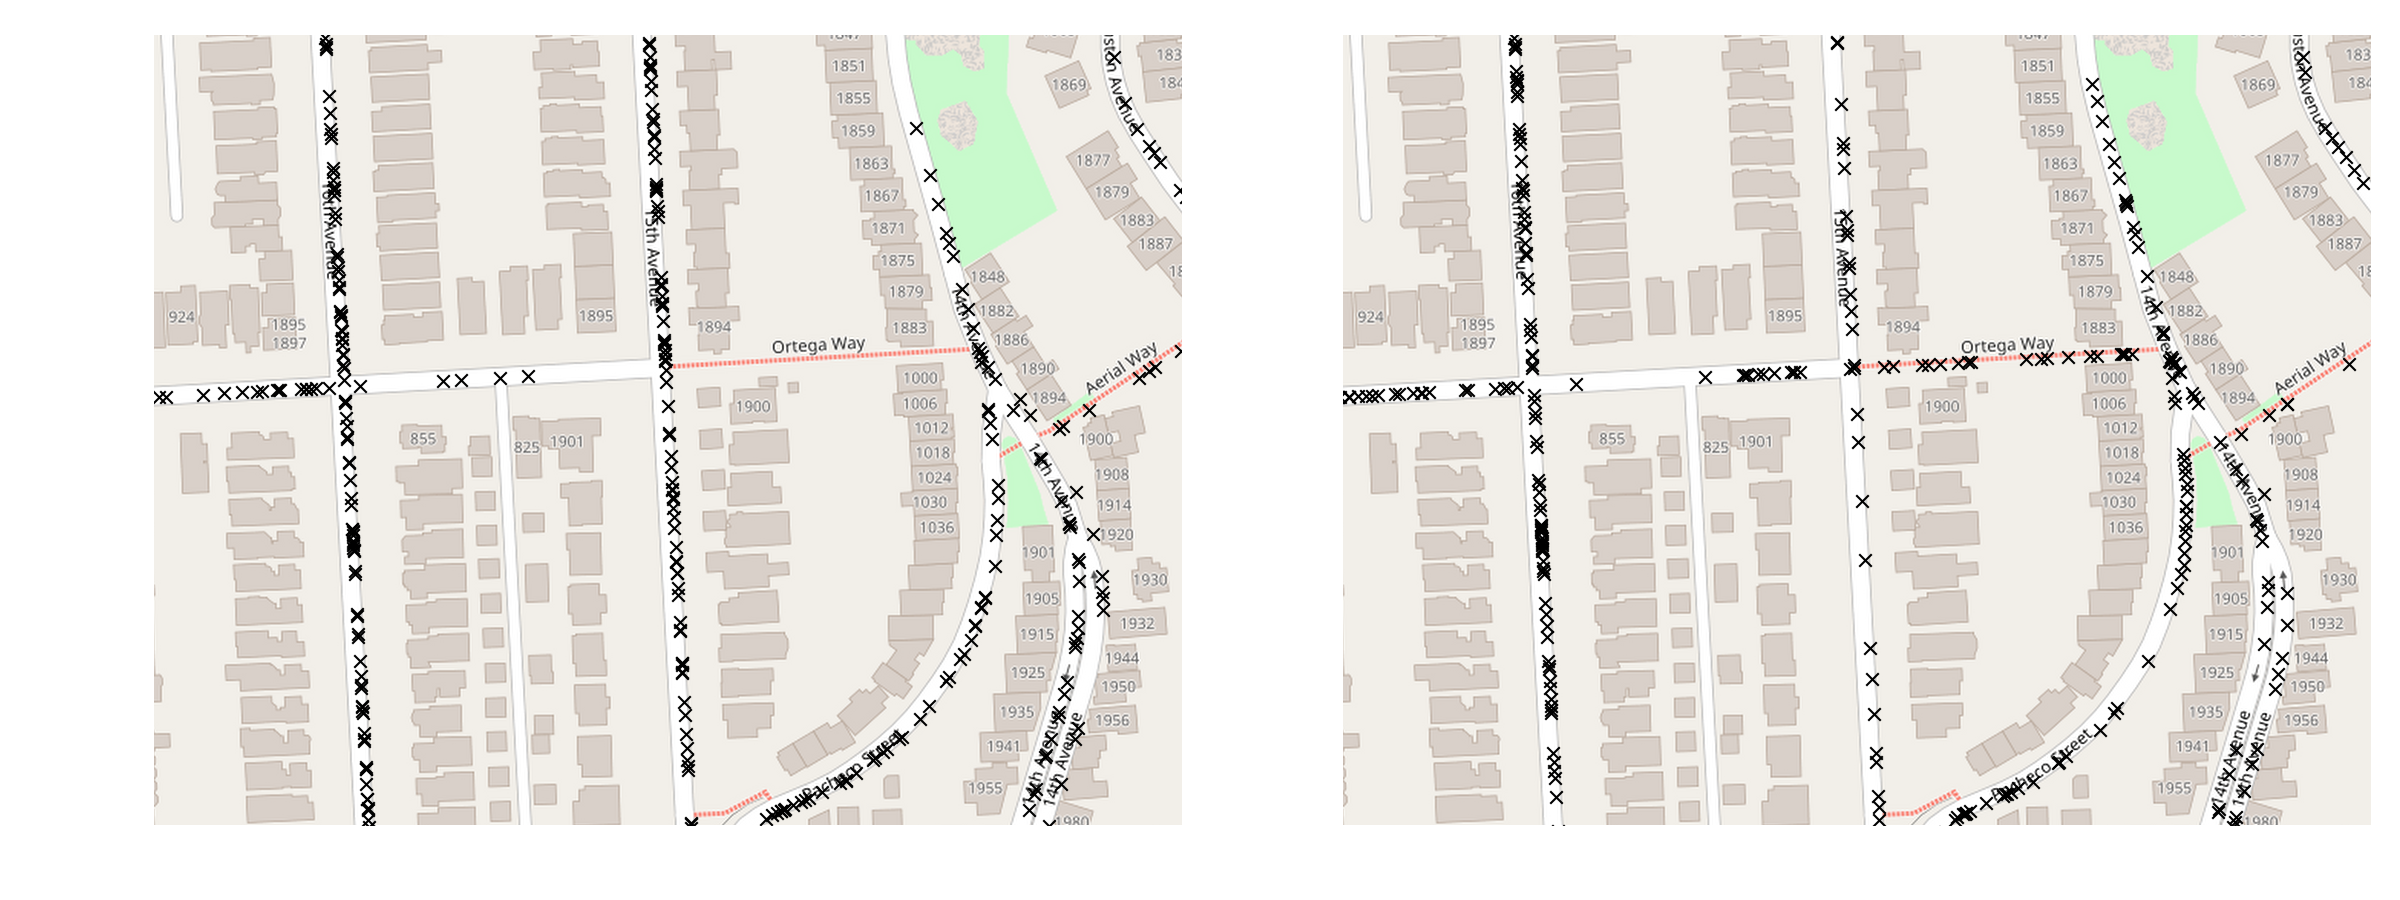
\includegraphics[width=\textwidth]{sf_redist_flow_network.png}
  \caption{Redistribution of points, as described in Section~\ref{sec:sf_flow}.
The left panel shows the result for the street network from \cite{sfgeo}, and the right
panel the result for the street network from \cite{tiger}.}
  \label{fig:sf_flow_redist}
\end{figure*}



\subsection{Assign to buildings}\label{sec:sf_assign_to_buildings}

We now use the building/address data from \cite{oa}.  Our algorithm takes the points,
as redistributed as in Section~\ref{sec:sf_flow} above, and then assigns the point to
the closest building/address in the database from \cite{oa}.

Initially, we experimented with assigning the point to the closest building.  However,
this often leads to a huge bias towards choosing buildings on one side of the street
(if the buildings are slightly closer to the street centre line).  In Figure~\ref{fig:sf_build_1}
we show (on the left) the results of instead assigning to a randomly chosen building.  We
first search within 75m of the point for a building; if we fail to find any, we double this
to 150m, then 300m, and so forth.  This leads to some unrealistic looking assignments.
On the right of Figure~\ref{fig:sf_build_1} we instead project the building locations to the
street network, and then search for nearby locations (firstly at 10m, then 20m, then 30m,
and so forth).  This gives a more visually pleasing result, whereby we assign a point to
a nearby building, without a bias to one side of the street or the other.

\begin{figure*}
  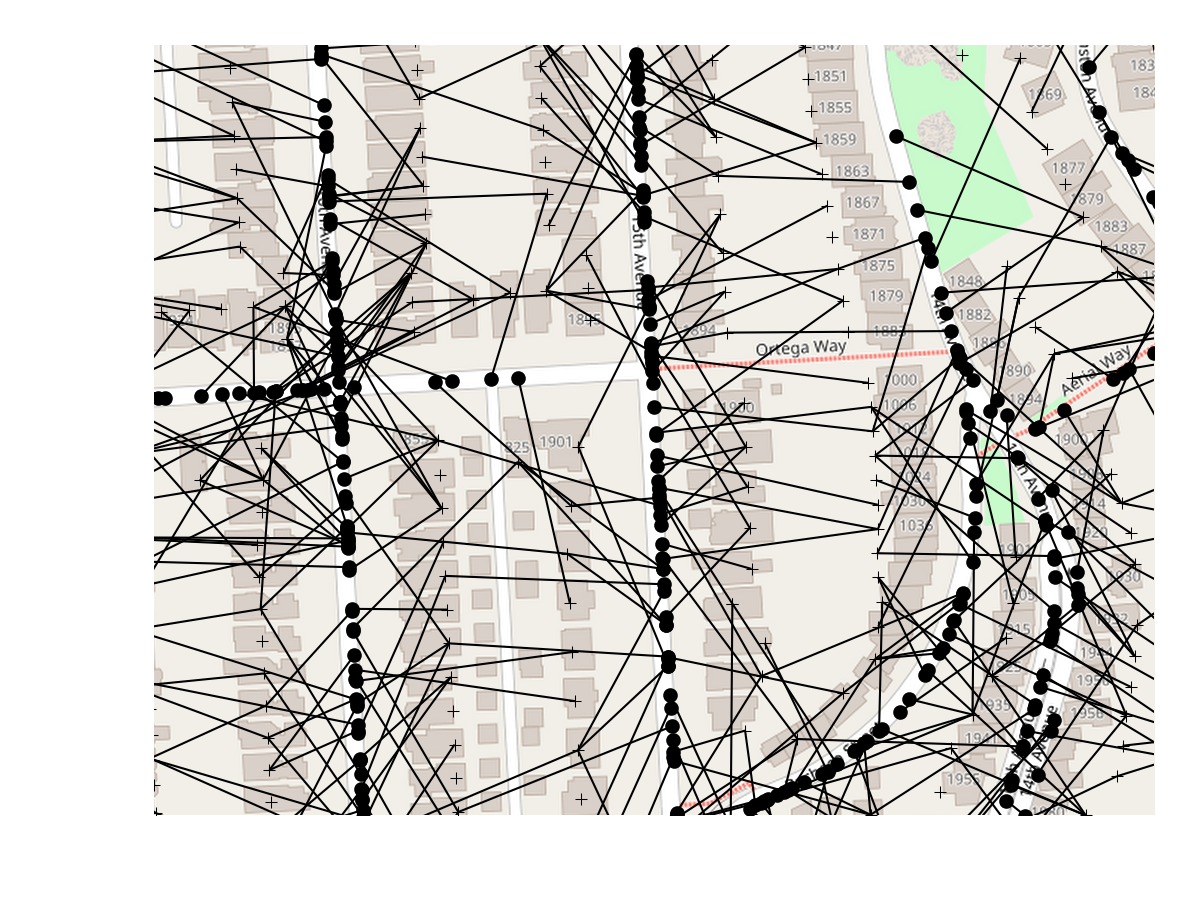
\includegraphics[width=3.2in]{sf_flow_to_buildings_1.png}
  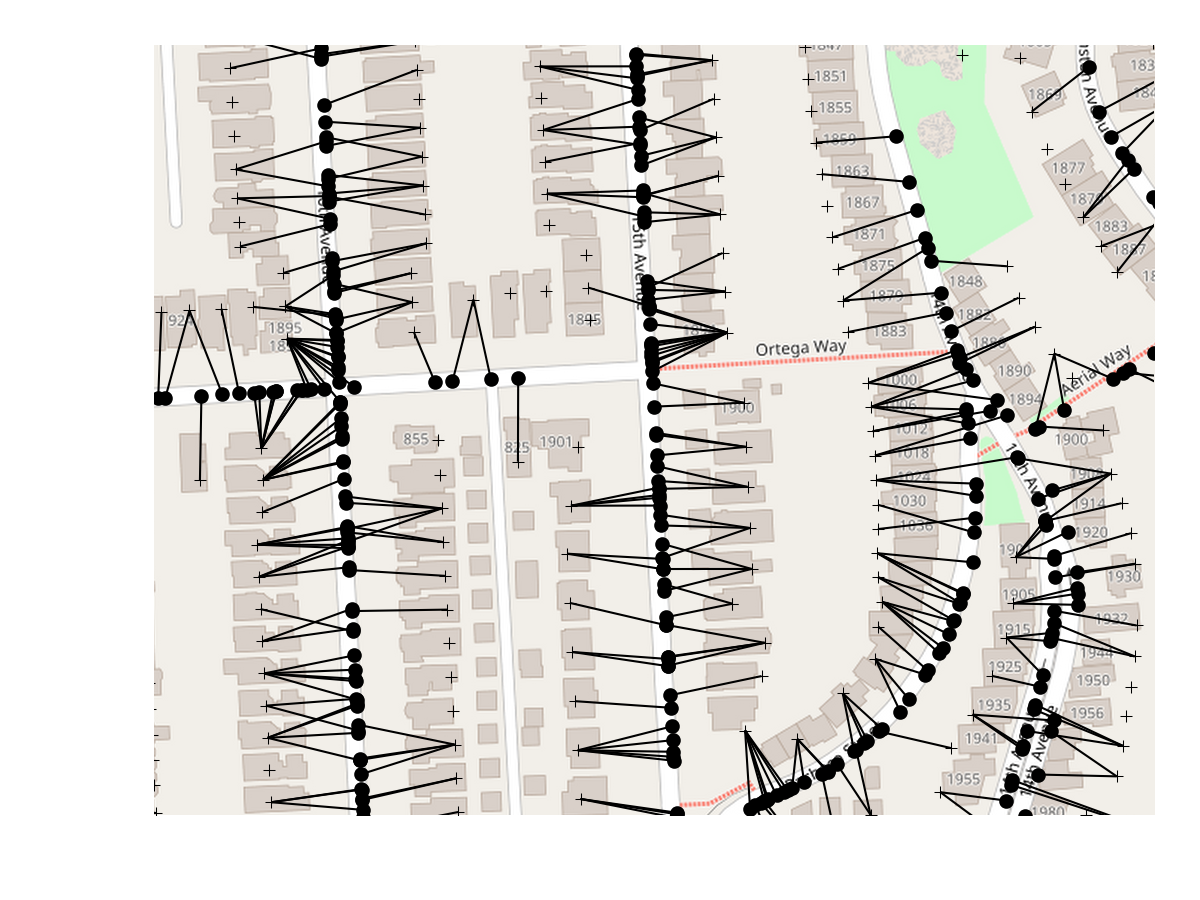
\includegraphics[width=3.2in]{sf_flow_to_buildings_2.png}
  \caption{Assigning the results shown in Figure~\ref{fig:sf_flow_redist} to the closest
  buildings in the database from \cite{oa}.  On the left, we assign at random to a building
  close (initial search within 75m) to the point assigned from Figure~\ref{fig:sf_flow_redist}.
  On the right, we project the building location to the network and then randomly choose
  a close point (initial search within 10m).}
  \label{fig:sf_build_1}
\end{figure*}



\section{Chicago}\label{chicago_redist_1}

We shall jump straight in, and use the street network from \cite{tiger} to form voroni cells.
We use the reduced street network (see Section~\ref{sec:link_st_net}) and form a voroni
cell around the mid-point of each edge in the network.  We then partition the network into
``segments''.  A segment is a maximal path where each interior node in the path has degree two.
That is, a segment is a section of the graph between two intersections.  We merge the voroni
cells corresponding to the edges in each segment.

Figure~\ref{fig:chicago_vor_2} shows the voroni cells so formed.  For the most part the
algorithm works well, capturing well the structure of the street network.  However, we do
end up with some rather small cells.  The shape of the cells is also quite dependent on
the number of edges in the original reduced graph: long straight streets will only use the
mid-point of a single edge, while a (slightly) curving street may consist of many edges, and
so ends up with a larger voroni cell.

\begin{figure*}
  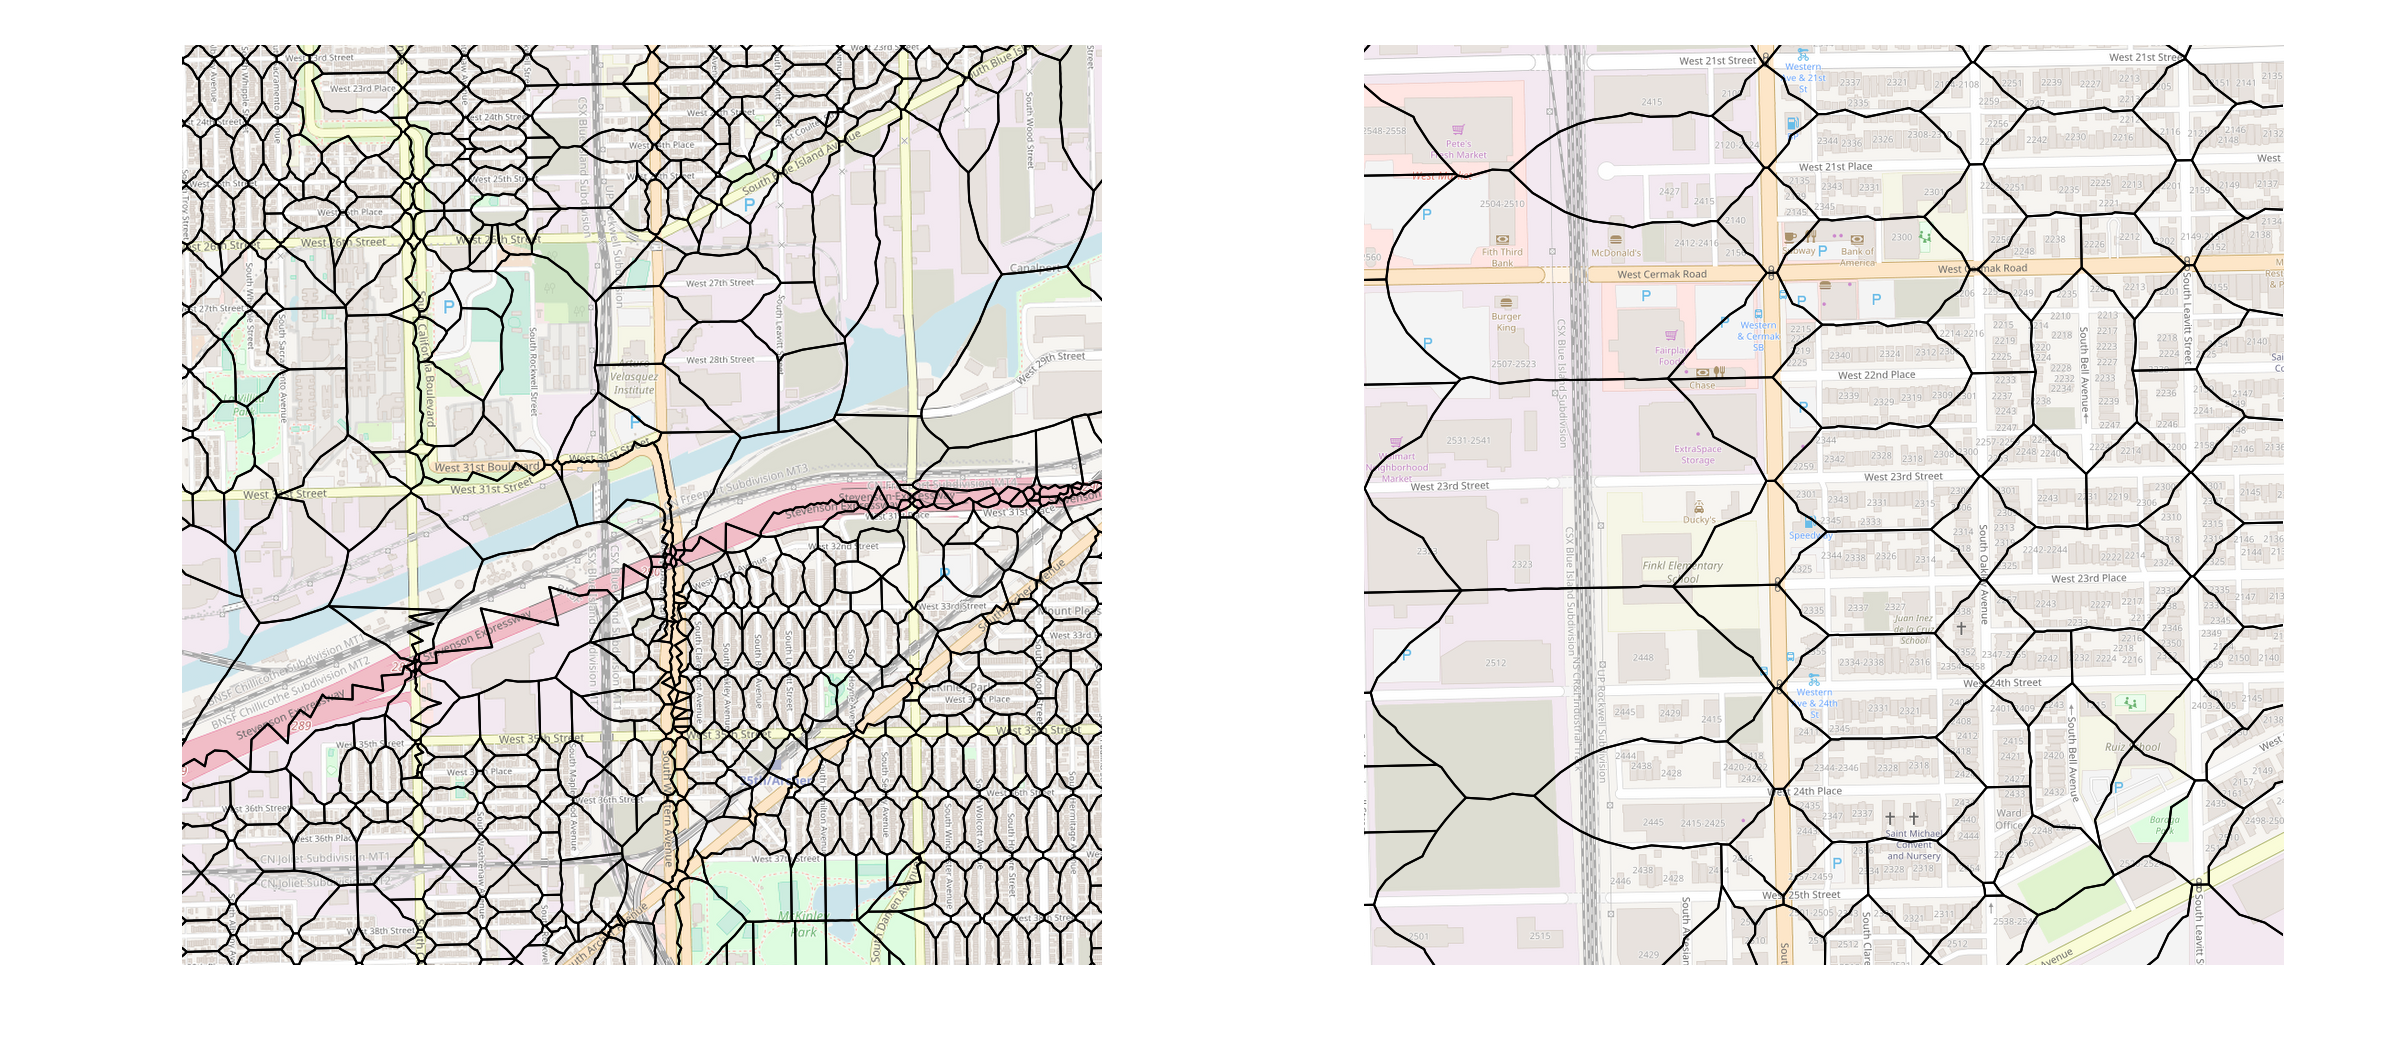
\includegraphics[width=\textwidth]{chiago_voroni_street_network_polys.png}
  \caption{Two examples of the voroni cells formed as in Section~\ref{chicago_redist_1} for Chicago.}
  \label{fig:chicago_vor_2}
\end{figure*}

Figure~\ref{fig:chicago_vor_1} shows the resulting assignment between old points and
new points.

\begin{figure*}
  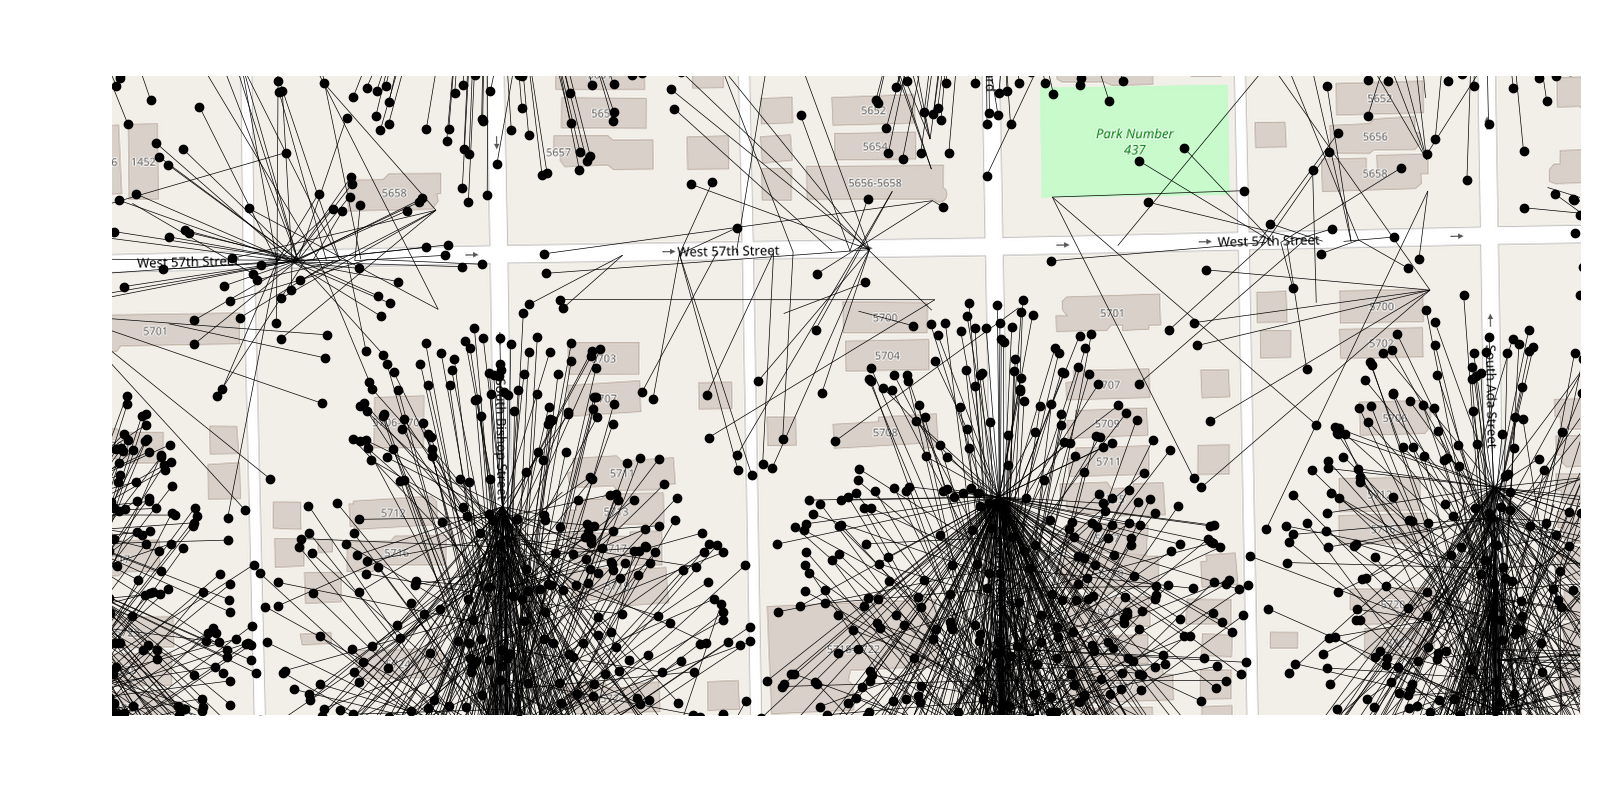
\includegraphics[width=\textwidth]{chicago_redist_network.png}
  \caption{Example of using voroni cells derived from the street network, for Chicago, to redistribute points.}
  \label{fig:chicago_vor_1}
\end{figure*}


\subsection{Use the clustering of the input data}\label{sec:chicago_vor_from_clusters}

The input data, Figure~\ref{fig:one}, shows very strong clustering, so it seems possible
that we could use this alone to form voroni cells.  We start by merging points which are
close together.  We perform this using a graph-based algorithm:
\begin{itemize}
\item Each point is a node of the graph;
\item We add an edge between any nodes which are within a maximum distance, here we use 10m;
\item We find the connected components of the graph, find the centroid of the nodes in
each component, and find the node which is closest to this centroid.
\item This node forms the ``merged points'' to which other points in this component are
assigned.
\end{itemize}
We then form a voroni cell around each ``merged point''.  Preliminary investigation of the
resulting cells showed that the cells were still quite small.  We merge voroni cells which
are:
\begin{itemize}
\item Adjacent to each other;
\item Small (less than $100\times 100 m^2$ in area);
\item Contain a small number of events from the total dataset (30 events)
\item If we look at the ``BLOCK'' string for each point which is assigned to the merged
point in the cells, then there is some overlap in the given blocks.
\end{itemize}
See Figure~\ref{fig:chicago_vor_3} for examples of the voroni cells thus formed.

\begin{figure*}
  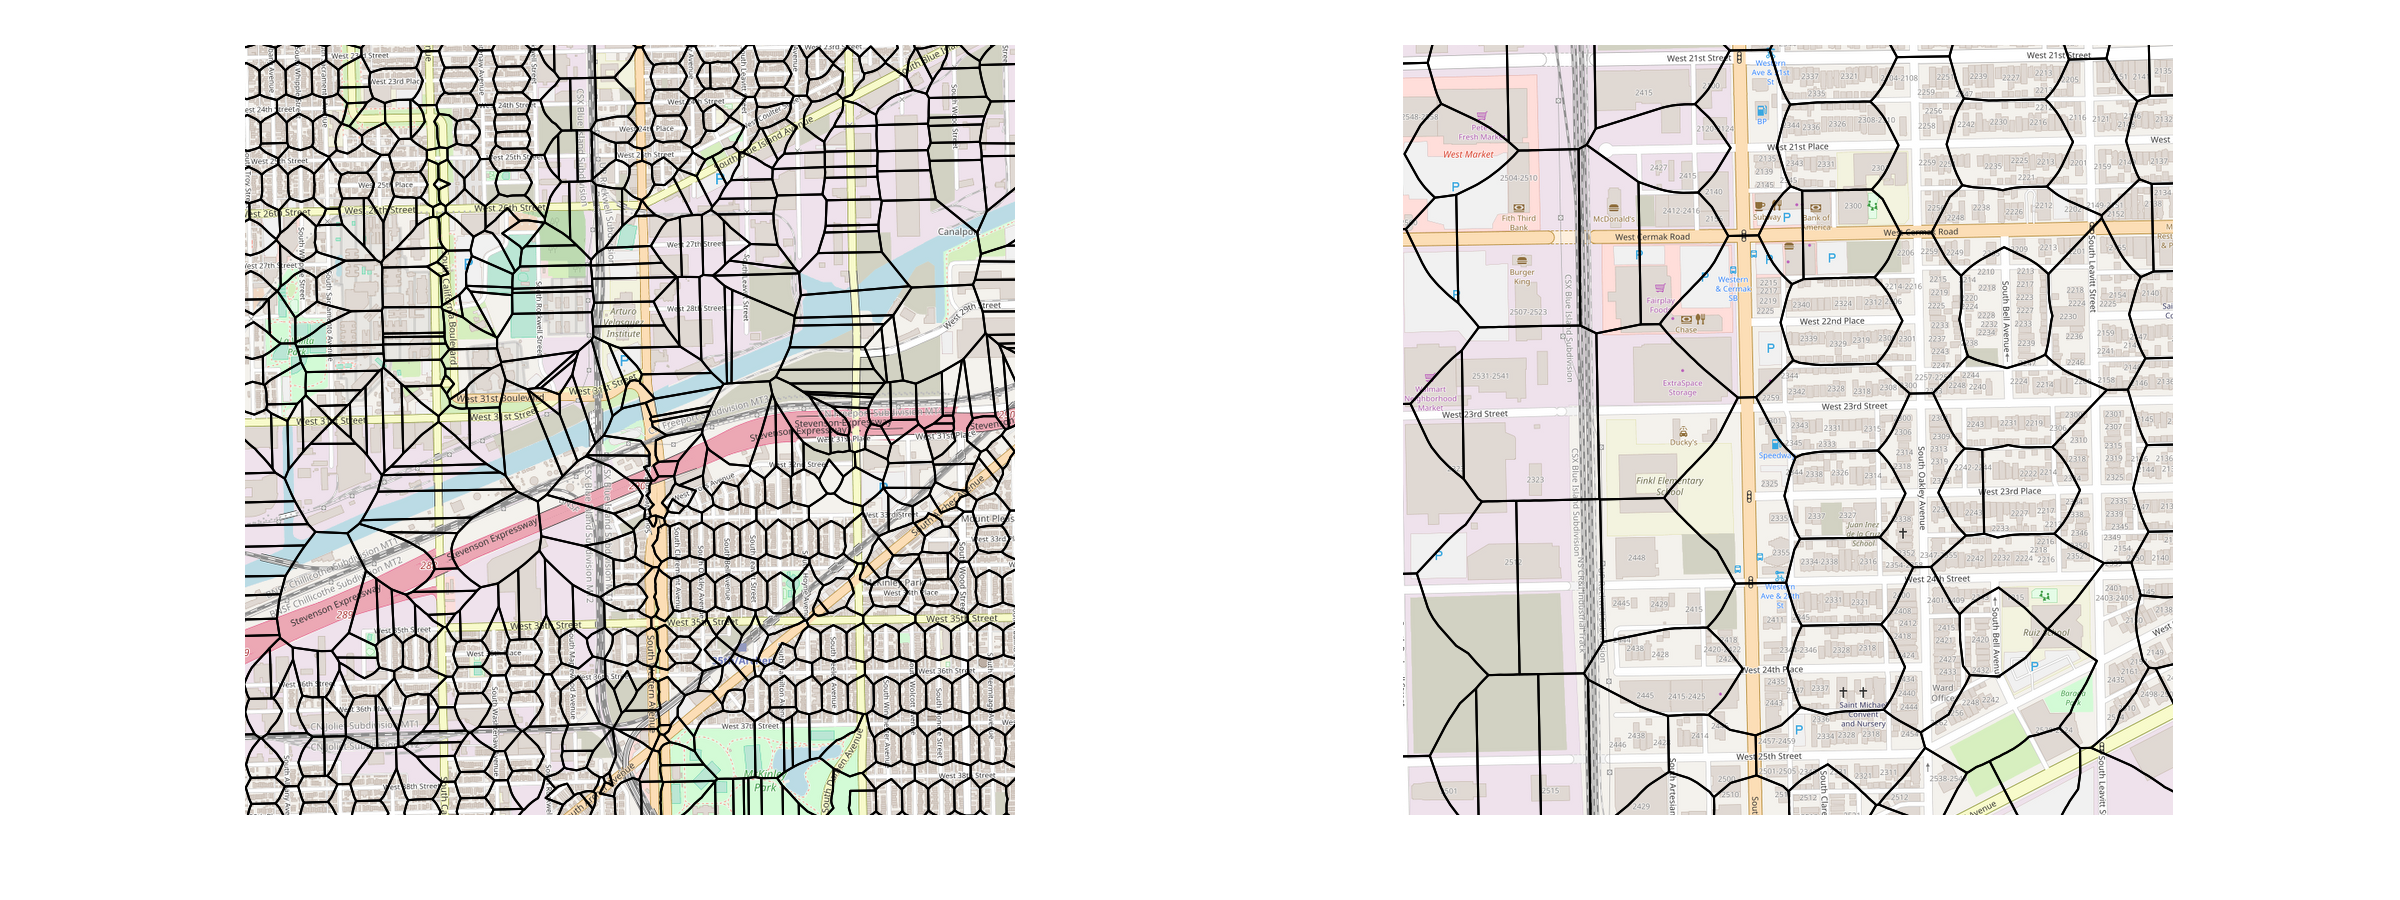
\includegraphics[width=\textwidth]{chiago_voroni_clustering_polys.png}
  \caption{Example voroni cells from the procedure given in
  Section~\ref{sec:chicago_vor_from_clusters}.}
  \label{fig:chicago_vor_3}
\end{figure*}

Figure~\ref{fig:chicago_vor_4} shows a resulting redistribution.  This looks similar to
Figure~\ref{fig:chicago_vor_1} but we see that points originally on the east/west streets
are distributed further.

\begin{figure*}
  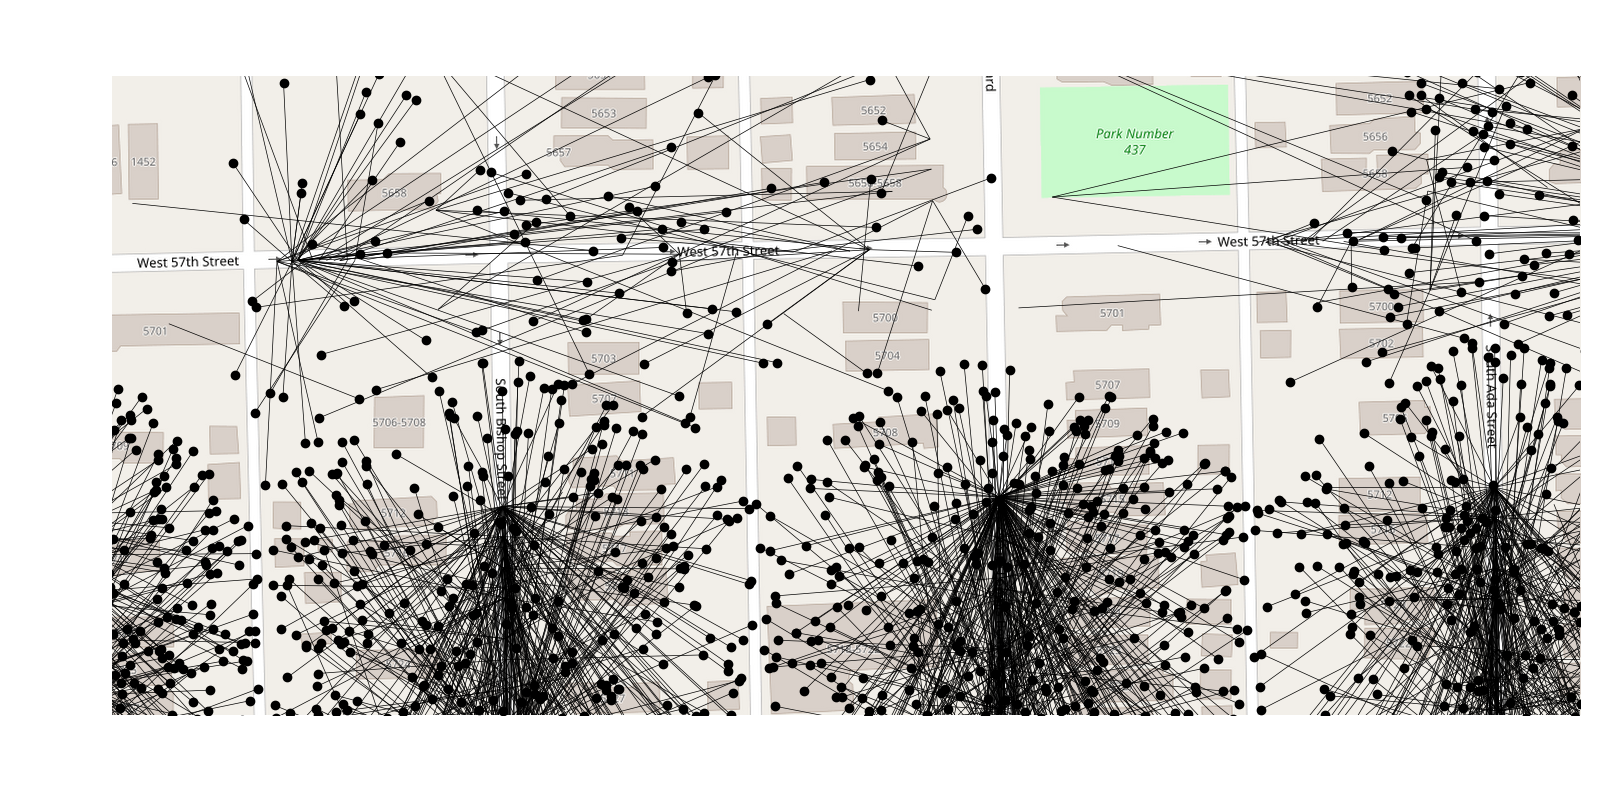
\includegraphics[width=\textwidth]{chicago_redist_cluster.png}
  \caption{Example of using voroni cells derived from clustering, for Chicago, to redistribute points.}
  \label{fig:chicago_vor_4}
\end{figure*}


\subsection{Using the network, and buildings}

We can proceed exactly as in Section~\ref{sec:sf_flow}, and use the street network data
from \cite{tiger} (forming the reduced network) and ``flow'' points around the network.
The results are very similar to those in Section~\ref{sec:sf_flow}, which is to be expected,
as again the vast majority of the input points already align with the street network, and
so we omit any plots.

We can similarly use the address / building information from \cite{oa}.  As the input points
for Chicago are not as highly aggregated as for San Francisco, it might be profitable to
assign input points to buildings directly.  We perform this as above, but now we choose the
closest building, and then choose at random any building (maybe the same one) within 100m
of the initial closest choice.  Figure~\ref{fig:chicago_buildings_1} shows the result.

\begin{figure}
  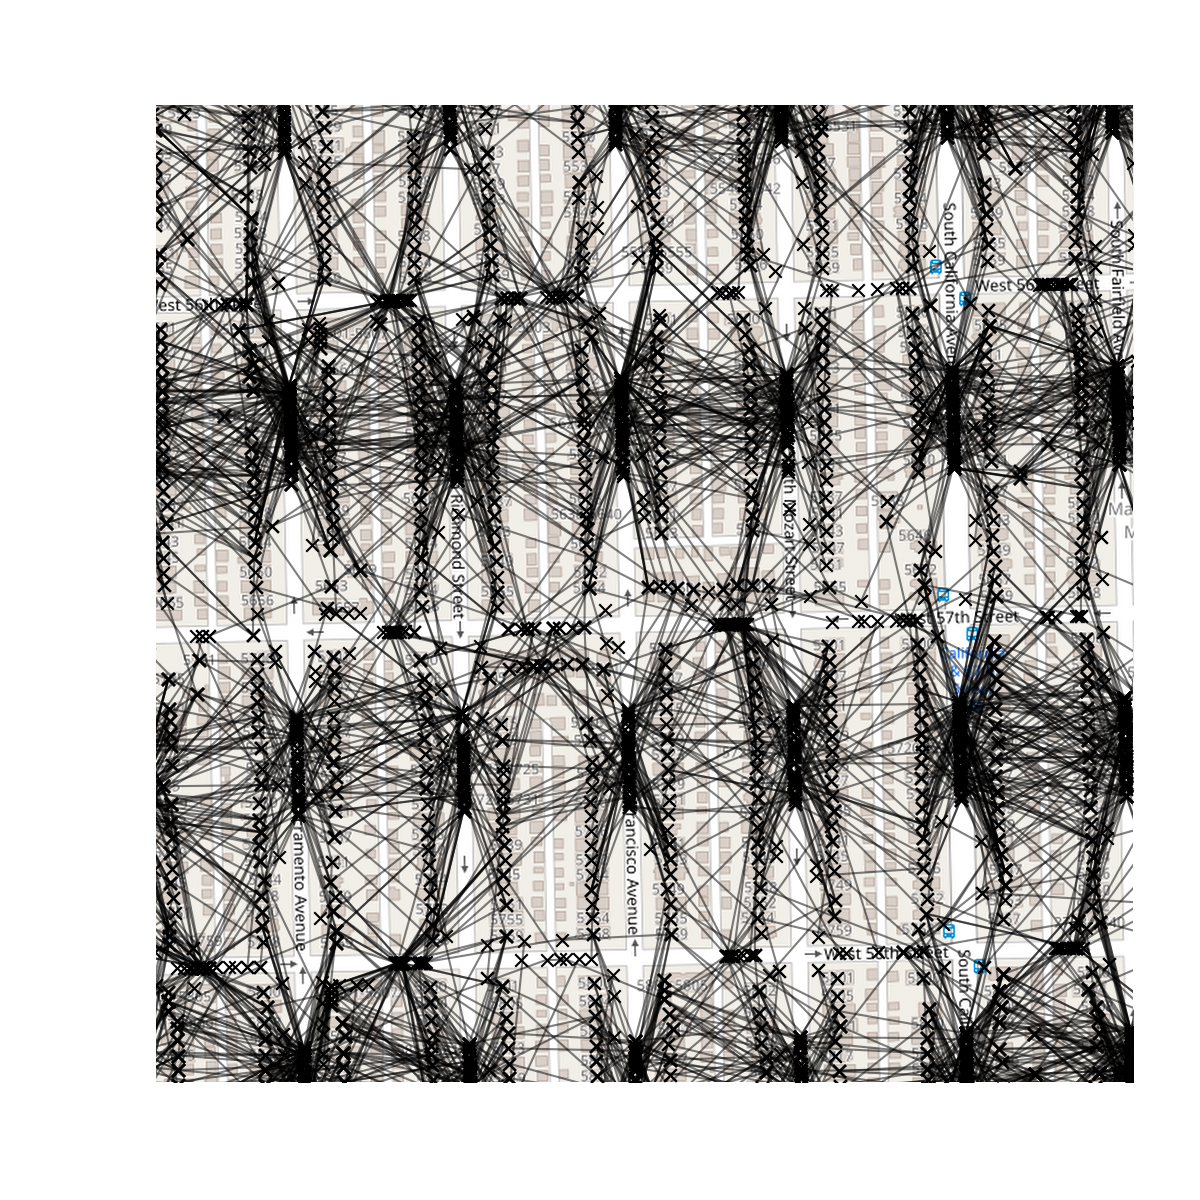
\includegraphics[width=3.5in]{chicago_buildings_1.png}
  \caption{Assigning the input point to a building location directly.  Initial and final
points are marked, together with a connecting line.}
  \label{fig:chicago_buildings_1}
\end{figure}

Finally, we can take the output of the ``network flow'' idea, and again assign
to a building, using the same algorithm as in Section~\ref{sec:sf_assign_to_buildings}.
This leads to Figure~\ref{fig:chicago_buildings_2}.  The left-hand plot here shows an
obvious weakness with the idea of using building / address data: if there are few (or only one)
building in an area, all events will be assigned to the same place.  However, if ``real world''
data is also geo-coded to addresses, then maybe this is ``realistic'', in the sense of
being similar to actual police data.

\begin{figure*}
  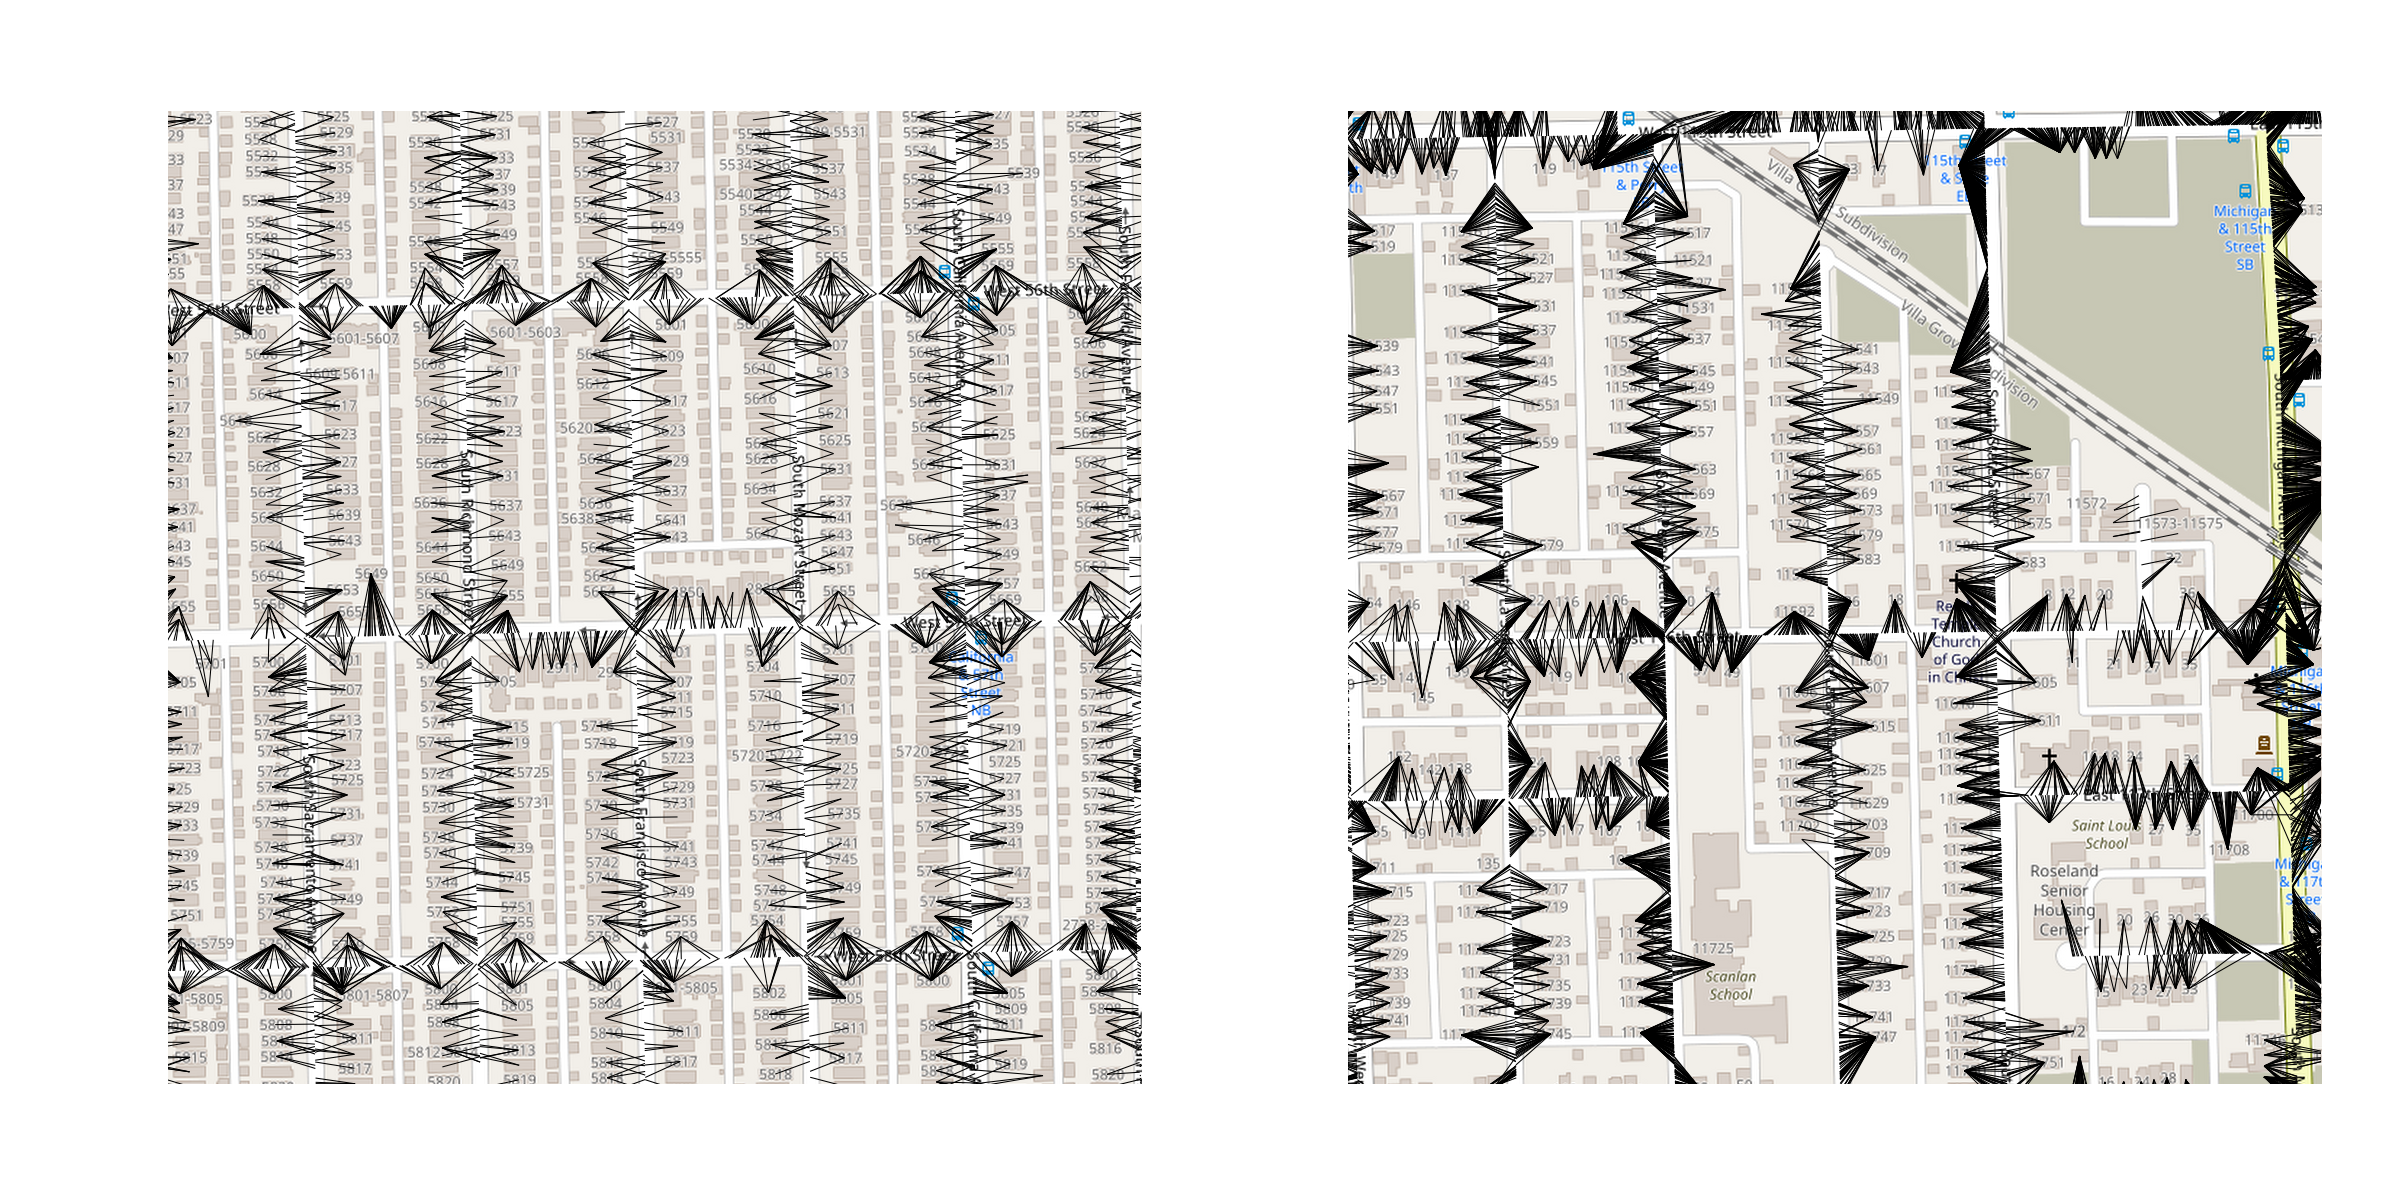
\includegraphics[width=\textwidth]{chicago_buildings_after_flow.png}
  \caption{Assigning the results of ``flowing'' points around the street network to
nearby buildings.  The left plot is the same basemap as Figure~\ref{fig:chicago_buildings_1};
the right plot is of an area with few address points.}
  \label{fig:chicago_buildings_2}
\end{figure*}



\section{Dallas}\label{sec:dallas}

The Dallas dataset presents a somewhat different problem, as for a subset of the data we
have accurate geocoding (projected to the street network), but for the overall dataset we
have coordinates which are seemingly somewhat randomly displaced from any notion of a
``correct'' placement.

We firstly try to use this partial data to ``guess'' a street network location for all the
points, as follows:
\begin{itemize}
\item We look at crime events only where we have both a longitude and latitude coordinates,
  and (seemingly randomly displaced) projected $x,y$ coordinates.  We ignore events where the two
  coordinates (after projecting using EPSG:2845) differ by more than 250m.  This latter
  step removes about 2.2\% of the data.
\item Project each longitude and latitude coordinate to the street network from
  \cite{dstreets}.  99\% of the input points are moved less than 8.4 meters by the operation.
\item We now form a Voroni diagram from the $x,y$ coordinates (merging those closer than
  1 meter apart).
\item We partition the street network into ``segments'' (compare Section~\ref{sec:link_st_net})
  and for each voroni cell, record which event gave rise to that cell (if there is a choice,
  take the first event) and so link each voroni cell to a street segment.
\item Now using the entire dataset, for each event we find the voroni cell which contains
  the $x,y$ coordinates, find the associated street segment, and then pick a point uniformly
  at random on that segment.
\item For those rows which have longitude and latitude coordinates, we move the vast majority
  of points between 1 metre and 1000 metres, most points moving less than 100 metres.  Given
  the random assignment, this suggests a good match.  However, there are certainly some
  outliers which are moved a long way.
\end{itemize}

From browsing the output data in QGIS, there are some mistakes, but also sometimes the matches
are quite surprisingly accurate (comparing by eye the location and the address data).
Figure~\ref{fig:dallas_to_streets} shows two example plots.

\begin{figure*}
  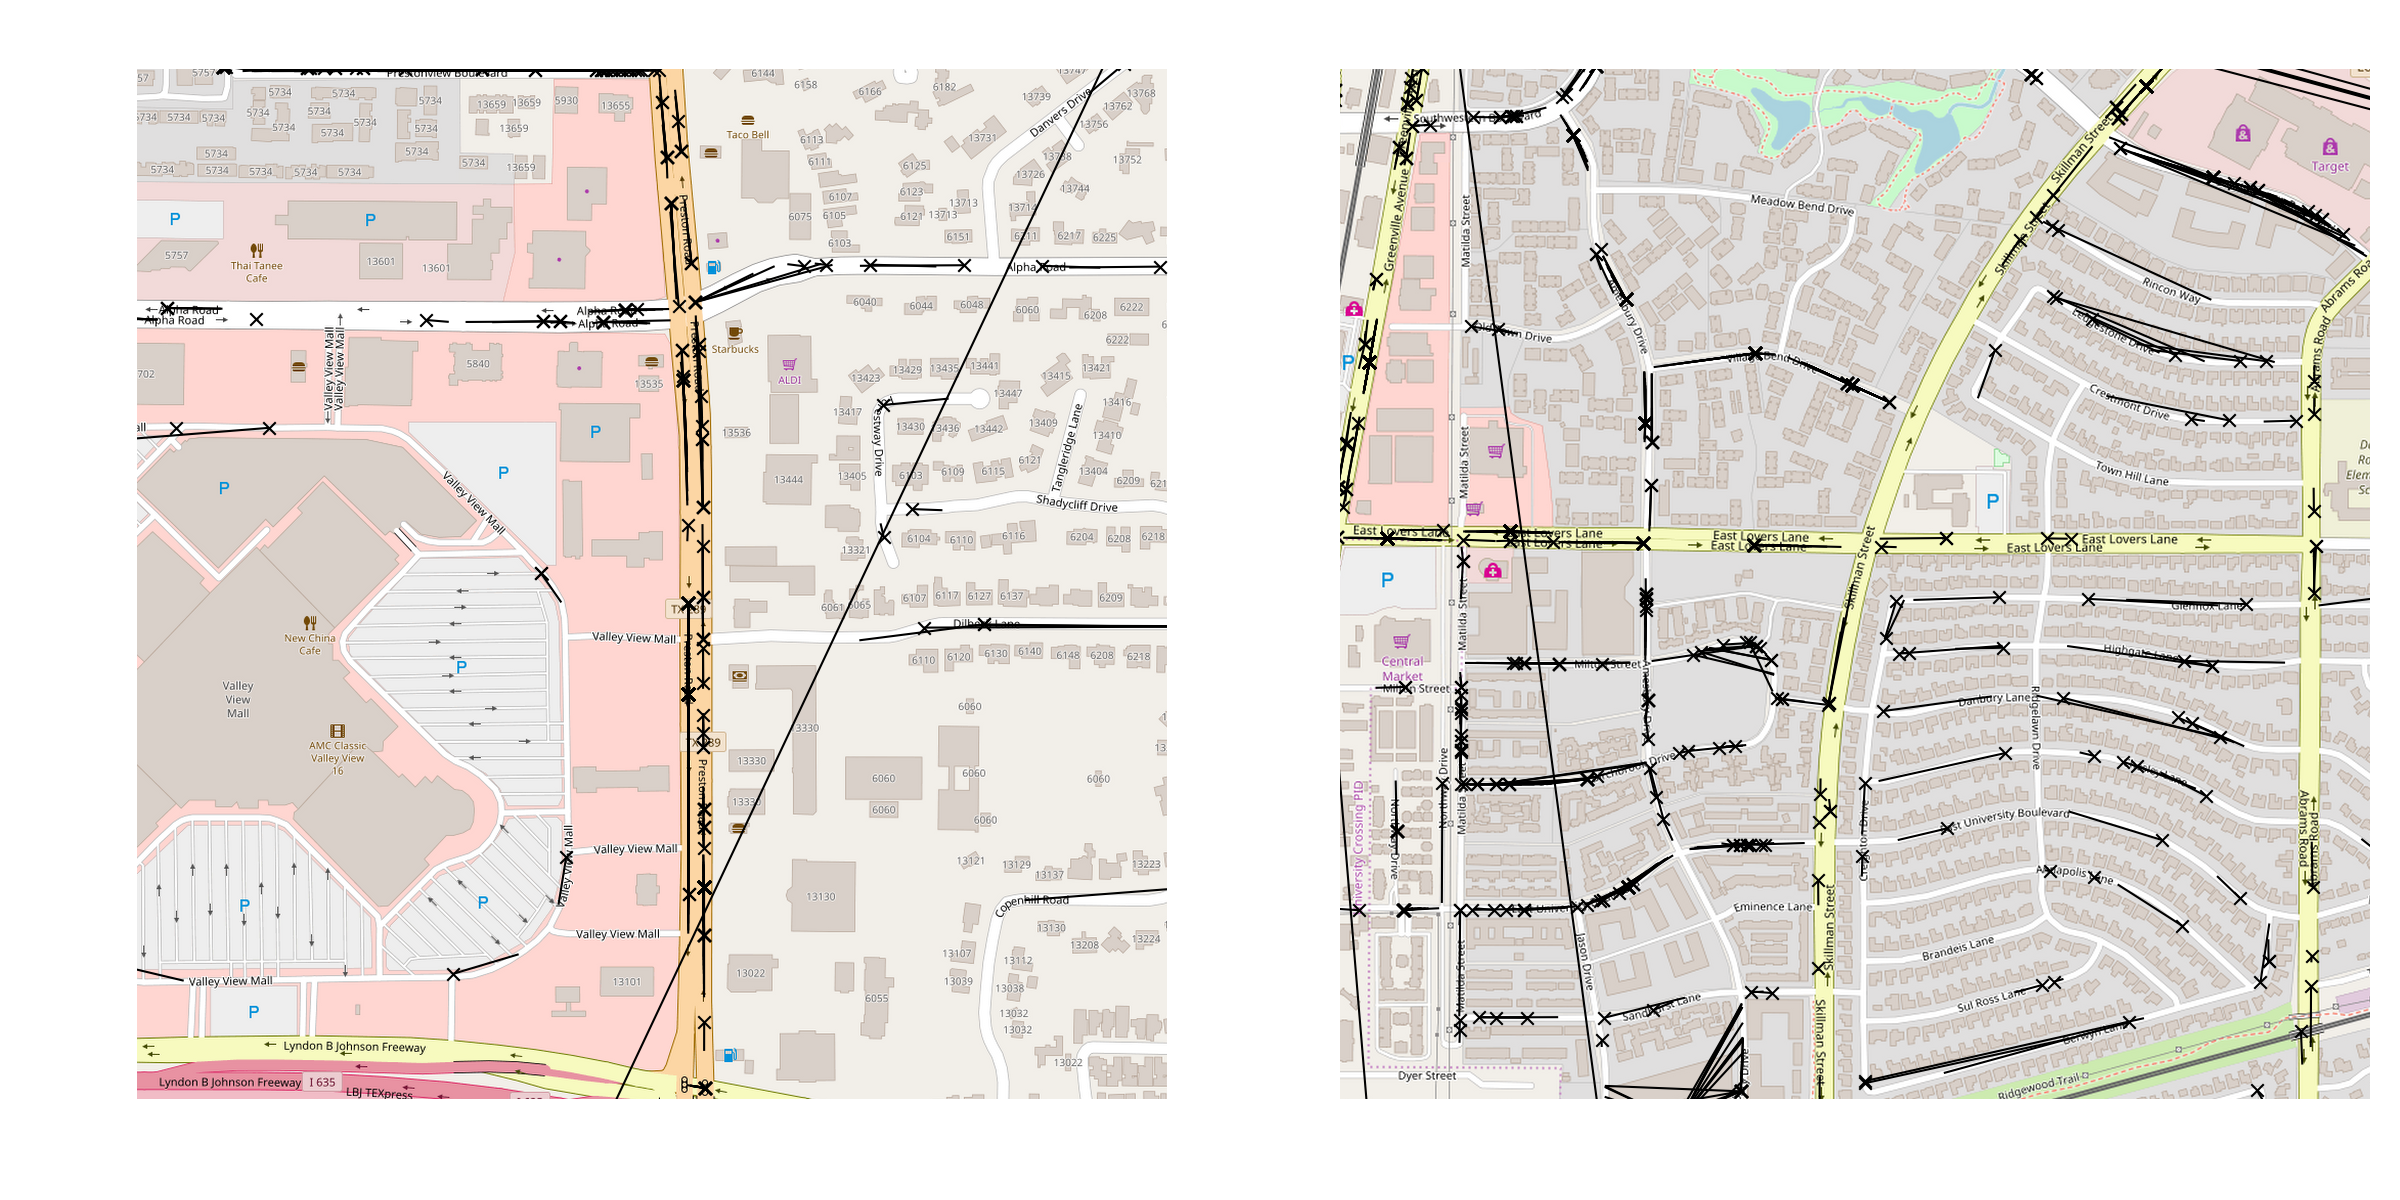
\includegraphics[width=\textwidth]{dallas_coords_to_streets.png}
  \caption{Assigning each Dallas event to the street network, as in Section~\ref{sec:dallas}.
Here we visualise only those events which originally had longitude and latitude coordinates,
plotted as $\times$, with a line connecting to the new street network location.}
  \label{fig:dallas_to_streets}
\end{figure*}

Finally we assign these new points to buildings, see Figure~\ref{fig:dallas_to_buildings}.
For the reasons explained in Section~\ref{sec:sf_assign_to_buildings},
we simply look at a disc around each point, initially of
radius 30m, and see if there are any buildings.  We increase the disc by 10m radius at a time,
until we do find a building.  If there is a choice, we pick one uniformly at random.
On the right of Figure~\ref{fig:dallas_to_buildings} we show a deliberately chosen difficult
case.  The majority of housing in this area (off Frankford Road) is gated communities, and the
address database (and OpenStreetMap) regard large numbers of distinct houses/apartments as being
the same address.  We thus assign many events to exactly the same location.  We note, however,
that the original longitude and latitude coordinates for these events are also identical:
they all have the same address, and geocode to the same point.  Thus, while the result is
obviously ``wrong'', there is quite some evidence that it might well be ``realistic'', in
the sense of corresponding to actual police data.

\begin{figure*}
  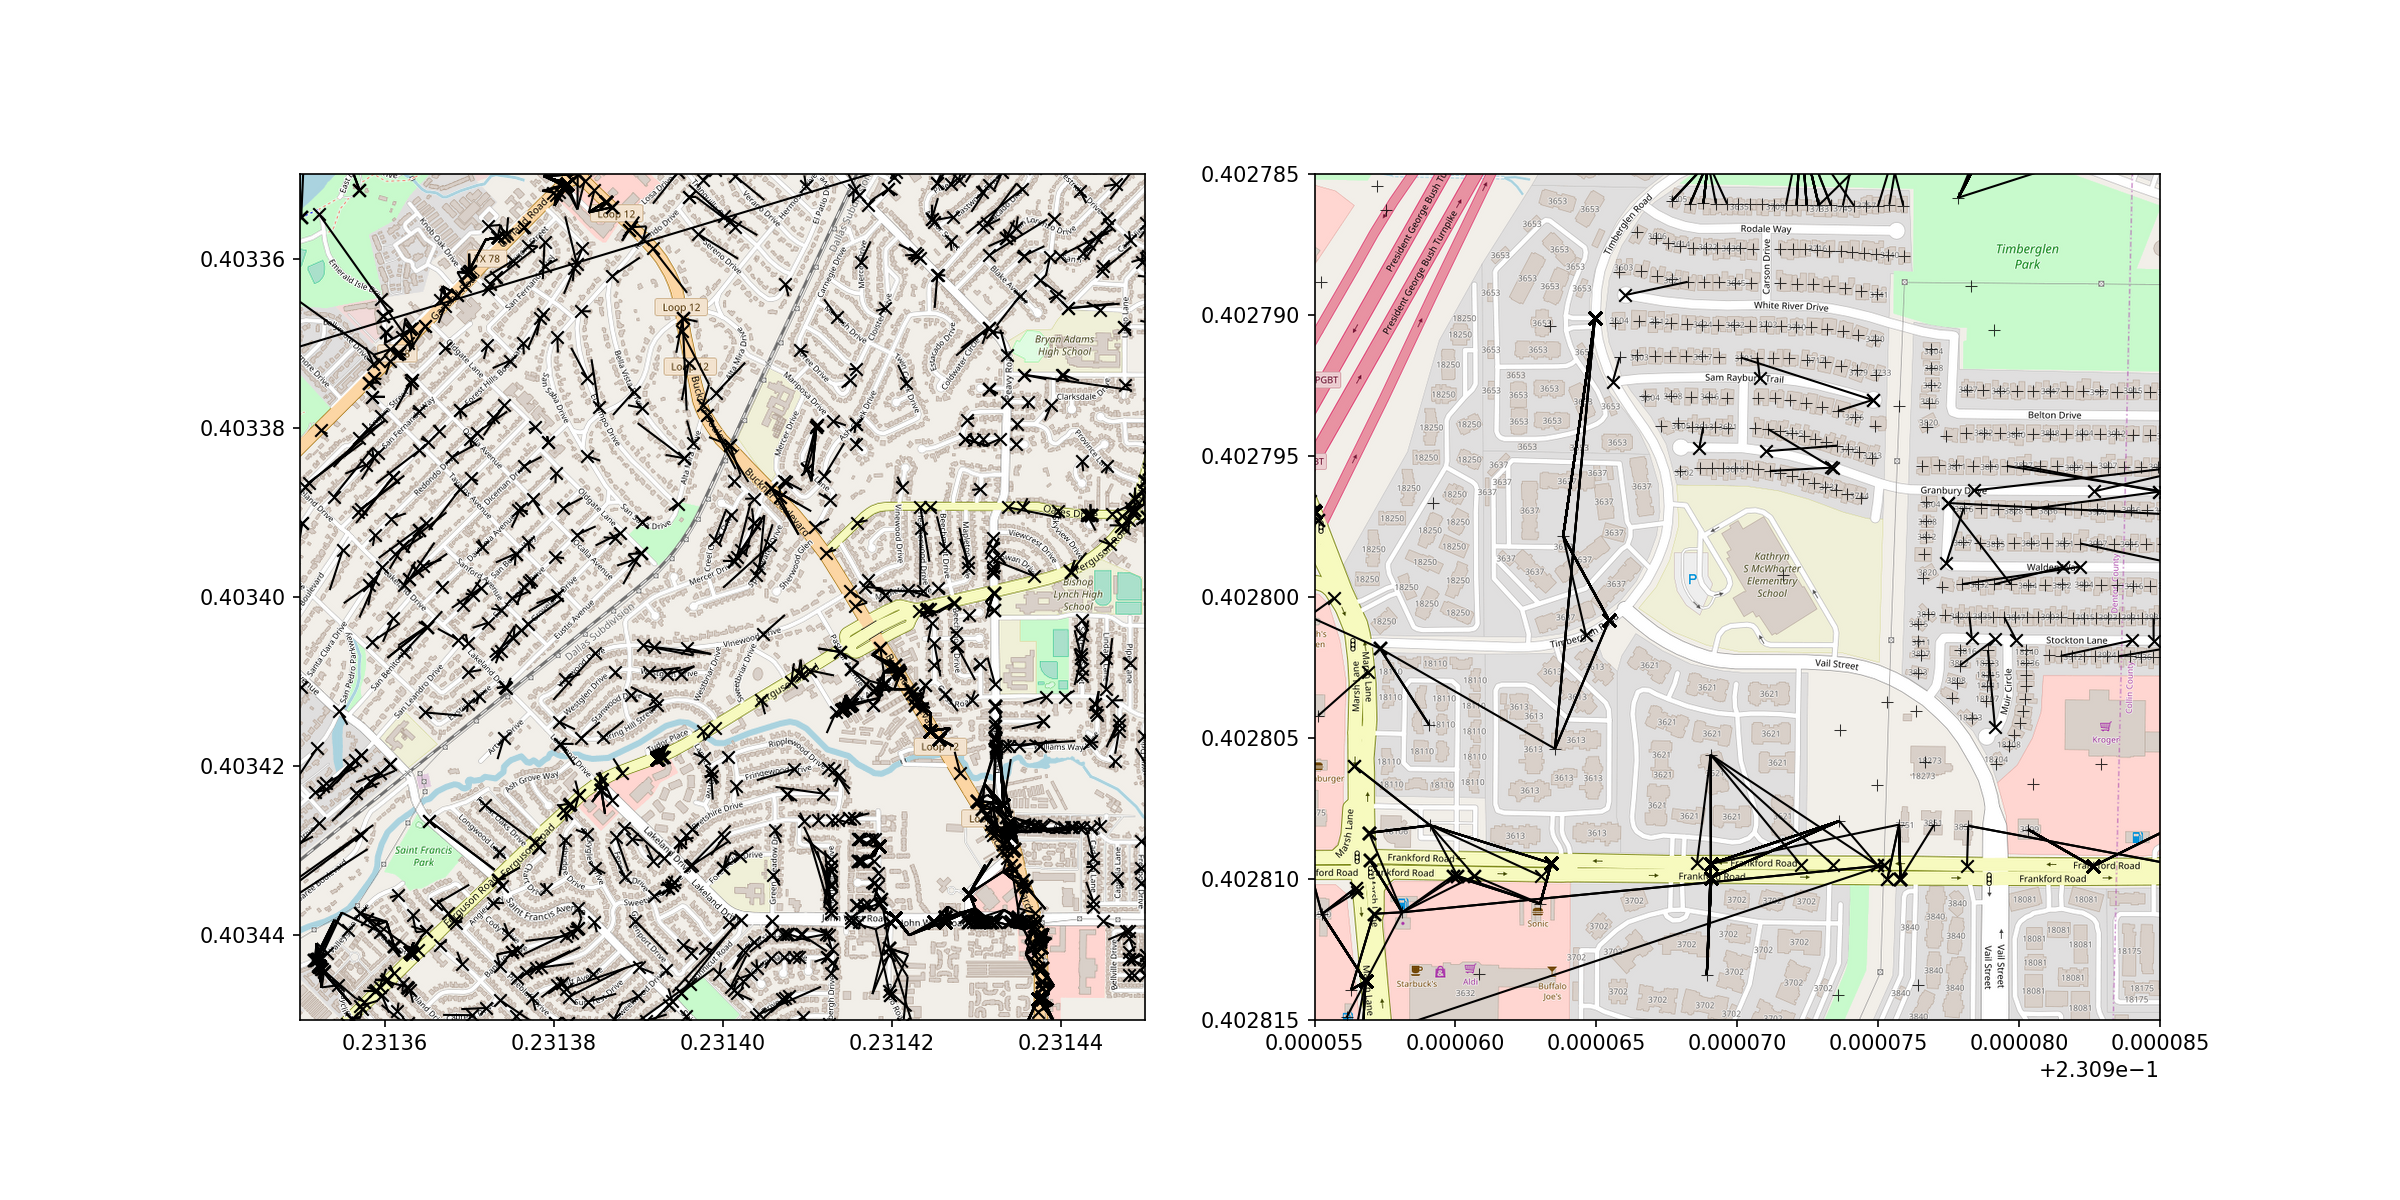
\includegraphics[width=\textwidth]{dallas_redist_to_buildings.png}
  \caption{Points redistributed from Figure~\ref{fig:dallas_to_streets} to the nearest
building / address.  We show only those events which have longitude and latitude coordinates;
a line joins the original and new locations; the original locations being marked with a
$\times$.  All buildings are marked with a $+$.}
  \label{fig:dallas_to_buildings}
\end{figure*}




\section{Conclusion: Making predictions}\label{sec:preds}

As an example application, we run some of the prediction algorithms developed in
\texttt{open\_cp} on both the original data, and some of the ``redistributed'' data.
In this case study, we use the South side of Chicago area, limit to just Burglary events,
and (for variation from
previously published studies) the data from 2007.  We use the data from January through
September 2007 as ``training data'', and then make predictions for each day, in turn, from
October through December 2007.  We note that an advantage of having an entirely automated,
scripted approach is that, if we wished to analyse a different time span, or a different
geographical area, we would literally need to change only a couple of lines of code, and
then re-run the scripts.

We show results for two prediction methods:
\begin{itemize}
\item The ``KDE'' method, which can be thought of as a ``modern'' prospective hotspotting
technique, compare \cite{bjp}.  We use a Gaussian KDE method for events in space, combined
with an exponential decay in time.  Compare with the description of the grid based method
in \cite{rosser_nw}.
\item The ``STScan'' technique, detailed in \cite{arc} for example.  This technique attempts
to find space-time cylinders which are experiencing an unexpected ``cluster'' of events.
\end{itemize}
For both methods, we use a grid of size 150m square, and the prediction technique ranks the
grid cells from most risky to least risky.  We then form a ``hotspot'' by selecting a
``coverage level'', say 10\%, and selecting the riskiest 10\% of grid cells.  Given the prediction,
we then score it by seeing how many of the actual crime events for the next day we ``captured''
inside our hotspot.  See \cite{arc, bjp} for more details of this by now standard methodology.

We statistically model this by treating each day independently, and assuming that the number of
captured events $n_i$ will be distributed as a Binomial out of $N_i$ total events, with chance
of success $\theta$ (independent of the day).  In \texttt{open\_cp} we implement a Bayesian
approach, using a Beta distribution for $\theta$, and then calculating the median of the posterior
distribution for $\theta$.  In practice, this will be close to the maximum likelihood estimation
for $\theta$, which is
\[ \hat\theta = \frac{\sum_i n_i}{\sum_i N_i}. \]
Notice that this is \emph{different} to simply calculating the mean of the daily ``hit-rates'',
which would be $\frac1k \sum_i n_i / N_i$; this is more commonly used in the literature, but
does not seem to fit a statistical model (it would tend to be biased if $N_i$, the total
number of events, varied greatly from day to day).

For both of these methods, there are various parameters (often termed ``bandwidths'') which can
be changed.  The choice of parameter is often not fully addressed in the literature, see
\cite{arc} for example, and compare the apparent novelty of using a MLE approach in
\cite{rosser_nw}.  We take a data-driven approach and try a variety of bandwidths, and
then select the one with the highest hit-rate (note that in other circumstances, this
could be criticised for mixing up ``training'' and ``evaluation'' datasets).  We use the same
settings across the datasets.

Figure~\ref{fig:hit_rates} shows the results.  We plot the hit-rate (as described above) against
coverage level.  We only extend to 20\% coverage level: if such hot-spots are ultimately
meant to inform police patrol plans, then selecting a large proportion of the study area as a
``hot-spot'' is fairly meaningless.

For the KDE predictor, we see that the original data gives a modest but notably higher
hit-rate.  This difference is certainly comparable to the differences between different
\emph{algorithms} as observed on the Chicago data in \cite{arc}.  This emphasises the point
that the \emph{exact nature} of the data might well be as important as the algorithm when it
comes to the hit-rate performance.  The ``STScan'' results are similar, but here we also
see a noticeable difference with the case when events are distributed to building performing
best.  It is interesting to note that this is the data we think most likely reproduces
``real-world'' police data (which is likely to be geocoded to individual addresses, at least
for events like Burglary).

\begin{figure*}
  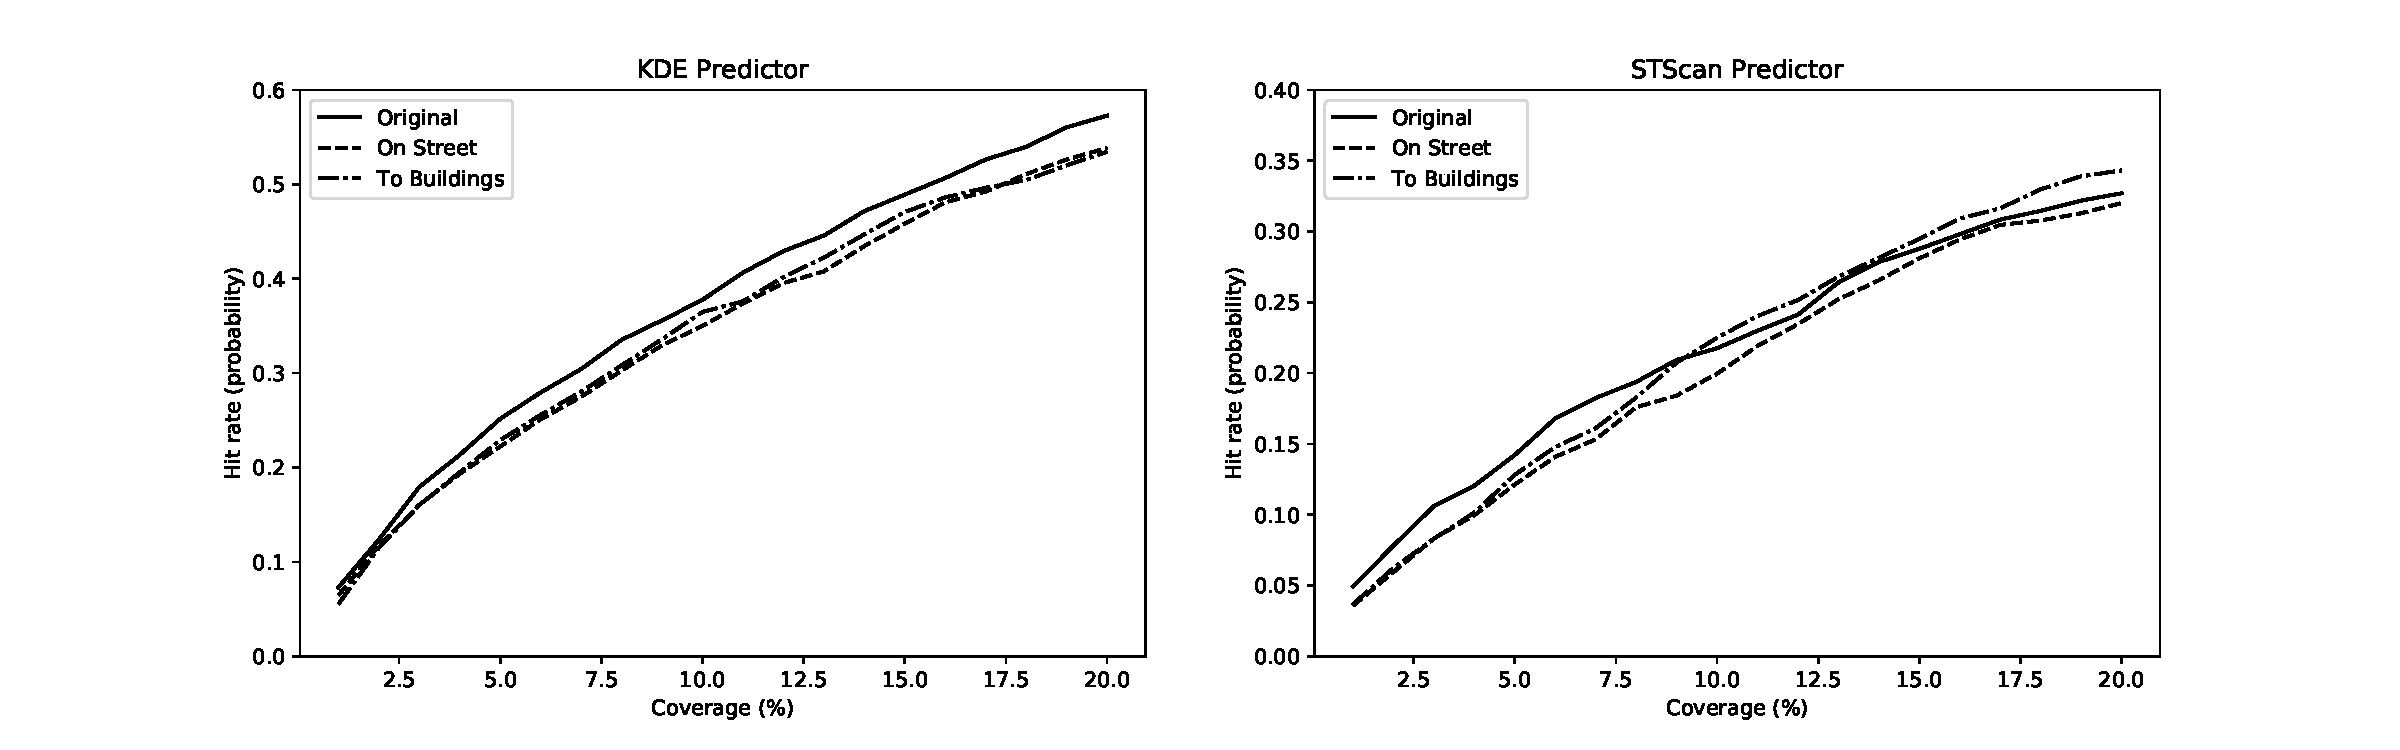
\includegraphics[width=\textwidth]{hit_rates.pdf}
  \caption{Hit-rate curves for two prediction techniques as applied to original data from
  the South side of Chicago, and two ``redistributed'' datasets.  See Section~\ref{sec:preds}.}
  \label{fig:hit_rates}
\end{figure*}


\subsection{Variability with grid offset}\label{sec:preds_grid}

We finish with a short exploration of how changing the grid \emph{offset}, but keeping all
other settings the same.  We use a variant of the prospective hot-spotting technique,
\cite{bjp}, with settings kept the same between datasets, on the same three datasets as above.
We compute the median hit-rate for 50 randomly chosen grid offsets, find the 5\% and 95\%
percentiles, and then report the difference.
Figure~\ref{fig:hit_rates_grid} shows how this difference in hit-rate
varies with coverage.  It is interesting to note:
\begin{itemize}
\item The slight positive correlation between coverage level and ``variability'' for
the two ``redistributed'' datasets; but the general lack of correlation for the original
dataset.
\item That, for low (and so possibly more ``realistic'') coverage levels, the two
``redistributed'' datasets show somewhat less variability than the original dataset.
\end{itemize}

Ideally, varying the grid \emph{offset} should have no effect upon the performance of
the algorithm: it should just be are arbitrary choice.  There is plenty of reason to suspect
that the interaction between an areal grid and data coming from a real geography might well
exhibit unexpected interaction.  It is hence interesting that the redistributed data seems
to behave in a ``better'' way than the original data.

\begin{figure*}
  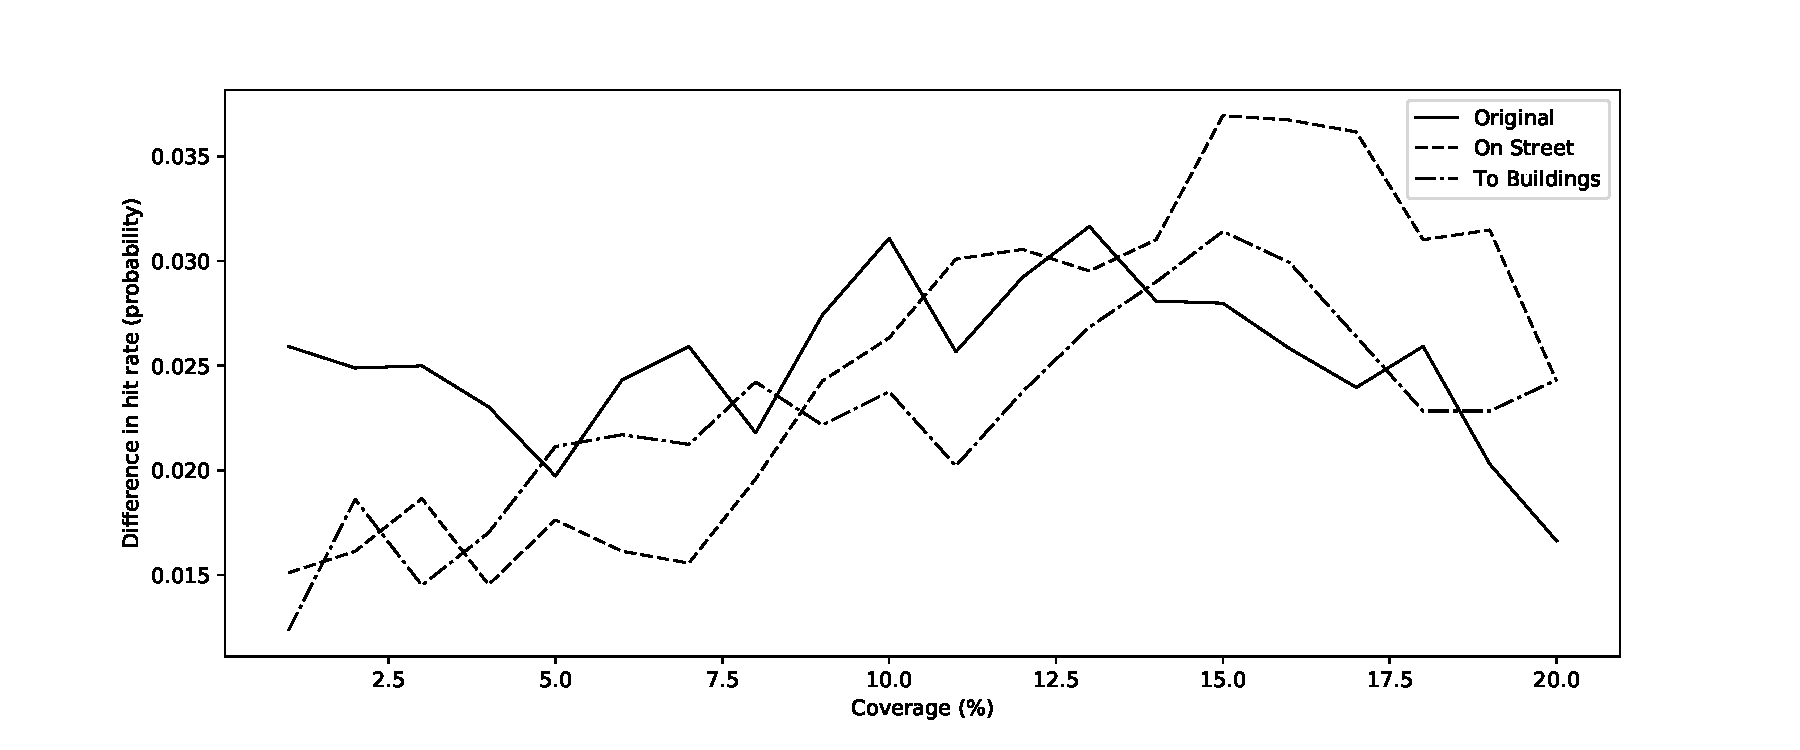
\includegraphics[width=\textwidth]{hit_rates_grid_vary.pdf}
  \caption{Difference in median hit rate between the 95\% percentile and 5\% percentile, at
  various hit rates.  See Section~\ref{sec:preds_grid}.}
  \label{fig:hit_rates_grid}
\end{figure*}



\begin{thebibliography}{99}

\bibitem{arc} M. Adepeju, G. Rosser, R. Cheng,
   ``Novel evaluation metrics for sparse spatio-temporal point process hotspot predictions - a crime case study'',
   International Journal of Geographical Information Science 30 (2016) 2133--2154.
   DOI: 10.1080/13658816.2016.1159684

\bibitem{barnes} N. Barnes, ``Publish your computer code: it is good enough'',
  Nature 467 (2010) 753.

\bibitem{beck} K. Beck, ``Test Driven Development: By Example''
  (Addison-Wesley Professional, 2002).

\bibitem{bjp} K.\,J. Bowers, S.\,D. Johnson, K. Pease,
	``Prospective Hot-Spotting.  The future of crime mapping?'',
	The British Journal of Criminology (2004) 44 641--658.

\bibitem{cdata} Chicago Data Portal, ``Crimes - 2001 to present'', available at
   {\small
   \texttt{https://data.cityofchicago.org/Public-Safety/} \texttt{Crimes-2001-to-present/ijzp-q8t2}}

\bibitem{cgeo} Chicago Data Portal, ``Boundaries - Community Areas (current)'', available at
   {\small\texttt{https://data.cityofchicago.org/Facilities-}
   \texttt{Geographic-Boundaries/Boundaries-Community-}
   \texttt{Areas-current-/cauq-8yn6}}

\bibitem{cstreets} Chicago Data Portal, ``Street Center Lines '' available at
   {\small
    \texttt{https://catalog.data.gov/dataset/street-}
   \texttt{center-lines}}

\bibitem{ddata} Dallas OpenData, ``Police Incidents'' available at
   {\small
    \texttt{https://www.dallasopendata.com/Public-Safety/}
   \texttt{Police-Incidents/tbnj-w5hb}}

\bibitem{dstreets} Dallas OpenData, ``Streets Shapefile'' available at
   {\small
    \texttt{https://www.dallasopendata.com/Geography-}
   \texttt{Boundaries/Streets-Shapefile-Polyline/}
   \texttt{cvgm-fp24}}

\bibitem{sfdata} DataSF, ``Police Department Incidents'' available at
   {\small
    \texttt{https://data.sfgov.org/Public-Safety/Police-}
   \texttt{Department-Incidents/tmnf-yvry}}

\bibitem{sfgeo} DataSF, ``San Francisco Basemap Street Centerlines'' available at
   {\small
    \texttt{https://data.sfgov.org/Geographic-Locations-}
   \texttt{and-Boundaries/San-Francisco-Basemap-}
   \texttt{Street-Centerlines/7hfy-8sz8}}

\bibitem{tmb} M. Daws, ``TileMapBase'',
   {\small\texttt{https://github.com/MatthewDaws/TileMapBase}}

\bibitem{ocd} M. Daws, ``OpenCrimeData'', open source Python library, available from
   \texttt{https://github.com/MatthewDaws/OpenCrimeData}

\bibitem{econ1} The Economist, ``Crime statistics in Chicago: Deceptive numbers'', published
  May 22nd 2014, see
  {\small\texttt{https://www.economist.com/blogs/democracy}
   \texttt{inamerica/2014/05/crime-statistics-chicago}}

\bibitem{eftelioglu} E. Eftelioglu et al. ``Mining Network Hotspots with Holes: A Summary of Results'',
  pp. 51--67, in ``Geographic Information Science.  9th International Conference, GIScience 2016, Montreal, QC, Canada'',
  Springer, 2016.

\bibitem{hlo} B. Harris, L. Larson, S. Ogletree,
  ``Different Views From The 606: Examining the Impacts of an Urban Greenway on Crime in Chicago'',
  Environment and Behaviour 50 (2018) 56--85.  DOI:10.1177/0013916517690197

\bibitem{HZ} T.\,C. Hart, P.\,A. Zandbergen,
  ``Effects of Data Quality on Predictive Hotspot Mapping'',
  NCJRS report 239861, September 2012, available at
  {\small
  \texttt{https://www.ncjrs.gov/app/publications/}
   \texttt{abstract.aspx?id=261934}}

\bibitem{hl} T. Hothorn, F. Leisch, ``Case studies in reproducibility'',
  Briefings in Bioinformatics 12 (2011) 288--300 DOI: 10.1093/bib/bbq084

\bibitem{morin} A. Morin et al. ``Shining light into black boxes'',
  Science 336 (2012) 159--160.

\bibitem{obs} A. Okabe, B. Boots, K. Sugihara,
  ``Spatial tessellations : concepts and applications of Voronoi diagrams'',
  (Wiley \& Sons, 1992.)

\bibitem{oa} OpenAddress, {\small\texttt{https://openaddresses.io/}}

\bibitem{odi} Open Data Institute, ``What is open data?'', available at
   {\small\texttt{https://theodi.org/what-is-open-data}}

\bibitem{osm} OpenStreetMap, ``Copyright and License'' available at
   {\small\texttt{http://www.openstreetmap.org/copyright}}

\bibitem{opencp} Quantitative Criminology at Leeds, ``\texttt{open\_cp}'',
   open source Python library, available at \texttt{https://github.com/QuantCrimAtLeeds/PredictCode}

\bibitem{qgis} Quantum GIS Development Team (2017).
  Quantum GIS Geographic Information System. Open Source Geospatial Foundation Project.
  {\small\texttt{http://qgis.osgeo.org}}

\bibitem{rand} W.\,L. Perry, B. McInnis, C.\,C. Price, S.\,C. Smith, J.\,S. Hollywood,
        ``Predictive Policing. The Role of Crime Forecasting in Law Enforcement Operations'',
        (RAND Corporation 2013).

\bibitem{ratcliffe} J.\,H. Ratcliffe, ``Aoristic analysis: the spatial interpretation of unspecific
temporal events'', International Journal of Geographical Information Science, 14:7, 669-679, DOI:
10.1080/136588100424963

\bibitem{rosser_sepp} G. Rosser, T. Cheng, ``Improving the Robustness and Accuracy of Crime
   Prediction with the Self-Exciting Point Process Through Isotropic Triggering'',
   Appl. Spatial Analysis (2016). DOI:10.1007/s12061-016-9198-y

\bibitem{rosser_nw} G. Rosser, T. Davies, K.\,J. Bowers, S.\,D. Johnson, T. Cheng,
   ``Predictive Crime Mapping: Arbitrary Grids or Street Networks?'',
   J Quant Criminol (2017) 33: 569--594. DOI: 10.1007/s10940-016-9321-x

\bibitem{ss} S. Shiode, N. Shiode,
   ``Microscale Prediction of Near-Future Crime Concentrations with Street-Level Geosurveillance'',
   Geographical Analysis 46 (2014) 435--455.  DOI: 10.1111/gean.12065

\bibitem{ssb} A.\,D. Singleton, S. Spielman, C. Brunsdon,
   ``Establishing a framework for Open Geographic Information science'',
   International Journal of Geographical Information Science (2016) 30:8 1507-1521.
   DOI: 10.1080/13658816.2015.1137579

\bibitem{tiger} United States Census Bureau, ``TIGER/Line\regsym Shapefiles'',
   available at
   {\small\texttt{https://www.census.gov/geo/maps-data/}
   \texttt{data/tiger-line.html}}

\bibitem{wilson} R. Wilson, Introduction to Graph Theory, fifth edition.
   (Prentice Hall, 2010).
   
\end{thebibliography}


\vspace{5ex}

\noindent\emph{Author's address:}
\parbox[t]{3in}{Jeremiah Horrocks Institute\\
University of Central Lancashire\\
Preston\\
PR1 2HE}

\bigskip\noindent\emph{Email:} \texttt{matt.daws@cantab.net}

\end{document}
